\documentclass[a4paper, 11pt]{report}
\usepackage[ngerman]{babel}
\usepackage[ansinew]{inputenc}
\pagestyle{headings}
\usepackage{graphicx}
\usepackage{wrapfig}
\usepackage[hyphens]{url}
\usepackage{etoolbox}
\appto\UrlBreaks{\do\a\do\b\do\c\do\d\do\e\do\f\do\g\do\h\do\i\do\j
\do\k\do\l\do\m\do\n\do\o\do\p\do\q\do\r\do\s\do\t\do\u\do\v\do\w
\do\x\do\y\do\z}
\usepackage{hyperref}
\usepackage{color}
\usepackage{multicol}
\usepackage{subfig}
\usepackage{pgfplots}
\usepackage{float}
\usepackage[T1]{fontenc}
\usepackage{textcomp}


%\pgfplotsset{
 % compat=1.9,
  %xlabel near ticks,
  %ylabel near ticks
%} 


\begin{document}

\begin{titlepage}
	\vspace{500mm}
	\begin{center}
		
		\textbf{
			\Huge{Praktikumsbericht}}
		\vspace{10mm}
		\textbf{
			\huge{Implementierung interaktiver Spiele auf mobilen Endger�ten}}
		\vspace{16mm}
		
		\begin{multicols}{2}{
				\Large{
					Patrick Gr�f
					
					Martin Groppe 
					
					Nils Geilen
					
					Alexandra Kaulfu�
					
					Malte Kremer
					
					Philipp Lambracht 
					
					Jonas Lenze
					
				}
			}
		\end{multicols}
	\end{center}
	\vspace{2mm}
	\begin{center}
		\Large{Betreuer: Stefan Scheglmann, Heinrich Hartmann}
	\end{center}
\end{titlepage}




\begin{abstract}
In der Vergangenheit konnte  zwischen virtuellen Spielen und Spielen in der physischen Welt klar unterschieden werden. 
Die gro�e Verbreitung von Mobiltelefonen mit hoher Rechenleistung, verschiedenen Sensoren und st�ndiger Internetverbindung erm�glicht es, Spiele zu entwickeln, die virtuelle und physische Umgebung vereinen.
In diesem Projekt soll untersucht werden, inwieweit es m�glich ist, traditionelle Bewegungsspiele mit einer App zu unterst�tzen oder klassische Videospiele ins Freie zu verlegen. Dazu werden Mehrspieler-Spiele entwickelt, die virtuelle Objekt in die tats�chliche Umgebung der Spieler integrieren und die so angereicherte Umgebung auf einem Mobiltelefon darstellen. 
Beim Spielen dieser Spiele sollen die Spieler direkt miteinander interagieren.
%Diese Anwendungen sollen auf direkte Interaktion zwischen Spielern aufbauen.
\end{abstract}
\newpage

% Inhaltsverzeichnis anzeigen
\tableofcontents

\chapter{Einleitung}
%Wir haben uns damit besch�ftigt Interaktivit�t zwischen Smartphones und den Benutzern herzustellen. Dazu nutzen wir verschiedene Sensorik, die uns solche Ger�te bieten.

%Was bedeutet Interaktivit�t f�r uns in diesem Zusammenhang? Wir wollen es schaffen die physische Umgebung in eine virtuelle Welt einflie�en zu lassen. Umgekehrt sollen Entscheidungen in der Realit�t von virtuellen Ereignissen unterst�tzt werden.


Durch die fortlaufende technologische Entwicklung vergr��ern sich M�glichkeiten und Qualit�t virtueller Realit�ten (\textit{virtual reality}, VR) stetig.
W�hrend VR meist f�r das Eintauchen in komplett synthetisch erzeugte Welten steht, ist \textit{augmented reality} (in etwa \glqq erweiterte Realit�t\grqq) eine Spielart der VR, bei der virtuelle Elemente in die tats�chliche Welt integriert werden \cite{azuma}. 
Smartphones bieten durch Ortungsfunktionalit�t und andere Sensorik die M�glichkeit, ihre Umgebung zu erfassen und durch virtuelle Elemente zu erweitern. Dadurch lassen sich interaktive Bewegungsspiele entwickeln, bei denen jeder Spieler durch sein Smartphone gleichzeitig geortet und mit Informationen �ber den Spielverlauf versorgt werden kann. Mobiles Internet macht es zus�tzlich m�glich, dass sich Smartphones der Mitspieler und Mitspielerinnen synchronisieren. Eine solche Interaktivit�t zwischen maschinengest�tztem Spiel und physischer Umgebung ist weder mit einem station�ren Rechner, noch mit einem nicht internetf�higen Handy m�glich.
Mehrspieler-Anwendungen, die versuchen eine erweiterte Realit�t mit dem Smartphone zu erzeugen sind vorhanden (siehe Abschnitt \ref{related}). Jedoch setzen nur wenige direkte Interaktion zwischen den Spielern um und erfordern keine st�ndige Aufmerksamkeit und Bewegung von den Spielern.


In diesem Praktikum wird Android als Plattform genutzt, um die Beispiel-App\-li\-ka\-tio\-nen (siehe Kapitel \ref{implementationen}) umzusetzen.  Alternativen w�ren iOS oder Windows Phone. Zweiteres hat einen zu geringen Marktanteil \cite{android} und die Entwicklung f�r iOS ist mit hohen Lizenzkosten verbunden.  

In den folgenden Kapiteln werden zun�chst verschiedene Ideen vorgestellt, wie man virtuelle Spiele in die physische Welt integrieren kann oder eine virtuelle Welt in traditionelle Bewegungsspiele eingebaut werden kann (siehe Kapitel \ref{ideen}). Danach werden Spielkonzepte genannt, die zur Umsetzung dieser Ideen ben�tigt werden (siehe Kapitel \ref{konzepte}). Es wird untersucht, wie sich diese Konzepte technisch umsetzen lassen (siehe Kapitel \ref{technisch}). Mit Hilfe der erarbeiteten technischen L�sungen werden einige Spielideen als Android-Apps umgesetzt (siehe Kapitel \ref{implementationen}).


\chapter{Spielideen}
\label{ideen}
\section{Umsetzung virtueller Spiele in der physischen Welt}

Unter einem virtuellen Spiel verstehen wir jene, die sich ausschlie�lich  auf einem Computer spielen lassen.
Es folgen eine Reihe virtueller Spiele, die sich f�r die Integration in die physische Welt eignen.
\subsection*{Snake}
Ein absoluter Klassiker, der fr�her auf keinem Handy fehlen durfte. 
%Gerade wegen der Popularit�t und Einfachheit recht interessant es in die physische Welt zu integrieren. 
In einem begrenzten Areal gilt es eine Schlange geschickt zu steuern. Es m�ssen Items eingesammelt werden, wodurch die Schlange w�chst. Au�erdem muss darauf geachtet werden, dass weder der Rand des Areals noch die eigene Schlange ber�hrt wird.


\begin{figure}[htbp]
  \centering
    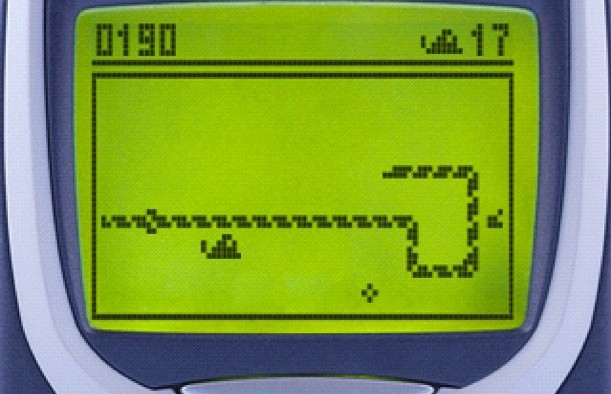
\includegraphics[width=0.5\textwidth]{2-Spielideen/2-1-Umsetzung_virtueller_Spiele_in_der_physischen_Welt/snake.png}
     \caption{Snake auf dem Nokia 3310 
		(Quelle: \url{http://nixtv.de/wp-content/uploads/2014/09/snake.jpg}) }
\end{figure}

Snake ist urspr�nglich ein Einzelspieler-Spiel. Da es un�blich ist, Outdoor-Bewegungsspiele allein zu spielen, haben wir entschieden Snake in der physischen Welt als Mehrspieler-Spiel umzusetzen, in dem wir als Spielfeld eine reelle Karte nehmen.  Wie wir dies umgesetzt haben, wird sp�ter erl�utert.

\subsection*{Capture the Flag}
Das Spiel ist nicht nur als virtuelles Spiel geeignet, wurde als solches aber erst richtig bekannt. Der relativ einfacher Spielmechanismus erleichtert den  Einsatz in der physischen Welt. Zwei Teams treten gegeneinander an. Jedes Team besitzt eine Basis mit einer Flagge, dessen Standort f�r das gegnerische Team bekannt ist. Es wird versucht die Flagge des jeweils anderen Teams zur eigenen Basis zu bringen. Gelingt dies w�hrend die eigene Flagge nicht vom gegnerischen Team "`entf�hrt"' wurde, erh�lt das eigene Team punkte. Wird eine gewisse Punktzahl erreicht, gilt das Spiel als gewonnen.

Problematisch im Falle einer Umsetzung ist, dass man in der Regel gegnerische Spieler "ausschalten" kann und diese dann in die eigene Basis zur�ckgesetzt werden. Dies muss im Fall einer Umsetzung anders realisiert werden.

Hilfreich bei der Integration in die physische Welt w�ren zum einen eine Richtungsangabe der Basis des gegnerischen Teams oder gar eine Karte, auf der die Basis angezeigt wird (eventuell auch die Position der eigenen Flagge, Position der Mitspieler, etc.), zum anderen der aktuelle Punktestand der Teams (eventuell mit Highscore).

\subsection*{Domination}
Meist in Kriegsszenarien integrierter virtueller Spielmodus, der sich mit wenig Aufwand in die physische Welt �bertragen l�sst. Zwei Teams treten gegeneinander an. Jedes Team hat einen Punktestand, der zu Anfang gleich ist, sich aber stetig verringert. Sinkt der Punktestand auf null, so ist das Spiel f�r dieses Team verloren. Es gibt verschiedene Areale, die eingenommen werden k�nnen. Ein Team kann ein Areal einnehmen in dem sich dort f�r einen gewissen Zeitraum mehr eigene Mitglieder als Mitglieder  des gegnerischen Teams befinden. Hierbei ist es m�glich gegnerische Spieler "auszuschalten". Diese starten dann wieder in einer Startzone. Auch hier m�sste dieses Spielelement im falle einer Umsetzung anders realisiert werden. Hat ein Team mehr Areale eingenommen als das Andere, l�uft der Punktestand des Teams, das weniger Areale in besitzt hat, schneller gegen Null.

 Verwirklicht werden kann das ganze, indem vor allem der Punktestand umgesetzt wird. Ebenfalls nicht unwichtig ist die Anzeige (z.B. auf einer Karte) der einzunehmenden Areale und in welchem Besitz sie sich gerade befinden. Au�erdem k�nnte dargestellt werden wo sich die eigenen Teammitglieder befinden.
\subsection{Integration einer virtuellen Welt in Bewegungsspiele}
Nat�rlich k�nnen wir die Integration auch von der anderen Seite betrachten. Es kann in
etablierte Bewegungsspiele der physischen Welt, eine virtuelle Umgebung eingef�gt
werden.
Ein paar simple BeiSpiele:
\subsubsection{Verstecken}
Es gibt eine Person, die der Suchende ist. Alle weiteren Mitspieler verstecken sich m�glichst
gut und versuchen vom Suchenden nicht entdeckt zu werden. Hat der suchende Spieler
alle Mitspieler gefunden ist das Spiel vorbei.
\subsubsection{Fangen}
Ein Spieler versucht alle anderen Mitspieler durch ber�hren zu �fangen�. Hat er geschafft
einen Mitspieler zu ber�hren ist nun dieser Mitspieler seinerseits dran einen anderen zu
fangen.
\subsubsection{Topfschlagen}
Ein Spieler bekommt die Augen verbunden. Er versucht anhand von Tipps der Mitspieler
(�n�her dran� oder �weiter weg�) einen Gegenstand zu finden.


\section{Related Work}
\label{related}
Wir sind nicht die Ersten, die mit einer Kombination aus realer und virtueller Welt experimentieren. Es gibt schon einige etablierte Spiele, die beides erfolgreich verbinden. Auch in anderen Bereichen, wie der Medizin  oder der Industrie, wird �ber die erweiterte Realit�t geforscht \cite{azuma}. 
% ?? H�ufig wird es im Sinne von viralem Marketing zur Bewerbung eines neuen Produktes oder einer neuen Dienstleistung verwendet, ohne dieses direkt anzupreisen und ohne das Spiel als Werbeveranstaltung erkennen zu lassen.
Im folgenden Abschnitt werden Spiele, die Teilaspekte der entwickelten Spielideen umsetzen, kurz erl�utert.

\subsubsection{Ingress}
%Google selbst l�sst sich nicht lumpen und hat ein erfolgreiches Spiel implementiert. 
Ingress \cite{ingress} ist ein kooperatives interaktives Gesellschaftsspiel, welches sich auf der ganzen Welt abspielt. Zu Anfang tritt ein Spieler eines von zwei Teams bei. Von nun an geht es darum, mit seinem Team, Kunstwerke, Bauwerke oder technische Landmarken virtuell zu kontrollieren. Diese werden im Spiel als Portale dargestellt. Spielern ist es m�glich kontrollierte Portale zu verlinken. Gelingt es drei Portale zu verlinken kann ein Dreieck Gebiet erzeugt werden, �ber welches das entsprechende Team dann "`herrrscht"'. Au�erdem will die sogenannte "`Exotic Matter"' eingesammelt werden. Dies geschieht beides mit dem Scanner, wie das Spiel seine App nennt. Wenn man mit dem Scanner in die N�he von "`Exotic Matter"' kommt, wird dies eingesammelt und es k�nnen Aktionen bei in der N�he befindlichen "`Portalen"' durchgef�hrt werden.

\begin{figure}[htbp]
  \centering
    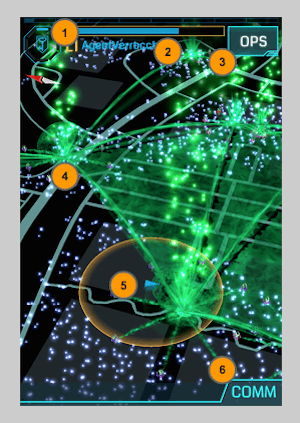
\includegraphics[width=0.5\textwidth]{2-Spielideen/2-3-Related_Work/ingress.png}
     \caption{der Scanner des Spiels Ingress. Auf der Karte werden "`Portale"' und das "`XM"' angezeigt und mit ihm k�nnen die Spieler untereinander agieren.
	(Quelle: \url{https://lh3.ggpht.com/OC9nlsdM9HjIUMJ4BHpUtLArV5qXyyqphqMHUjsmXp82rYcmSJgcp4v5DmXI5R7eB2z1fckH=w300})
		}
\end{figure}


\subsubsection{Pacman auf Google-maps}

%Ein weiteres kleines Minispiel, welches sich Google hat einfallen lassen, lie� sich nur eine bestimme Zeit lang spielen. 

Um den 1. April 2015 konnte man auf der normalen Google-Maps Seite die Stra�enkarte in ein Pacman-Spiel \cite{pacman} verwandeln und sich somit durch seine eigene (virtuelle) Stadt mit dem kleinen gelben Kreis fressen. 
Dies ist zwar nur ein Videospiel, dass vollst�ndig virtuell (ohne aktive Bewegungen in der Realit�t) gespielt wird, jedoch wird hier eine reale Karte als Spielfeld verwendet, was in unseren Implementationen ebenfalls ein wichtiger Punkt ist.
 
%Dies ein eher simples Beispiel f�r die Einf�hrung der realen Welt in ein virtuelles Spiel, da hier lediglich die Stra�enkarten in das Spiel integriert wurden. �hnlich den erarbeiteten Spielideen werden bei dieser Anwendung virtuelle Objekte auf einer Karte angezeigt.

\begin{figure}[htbp]
  \centering
    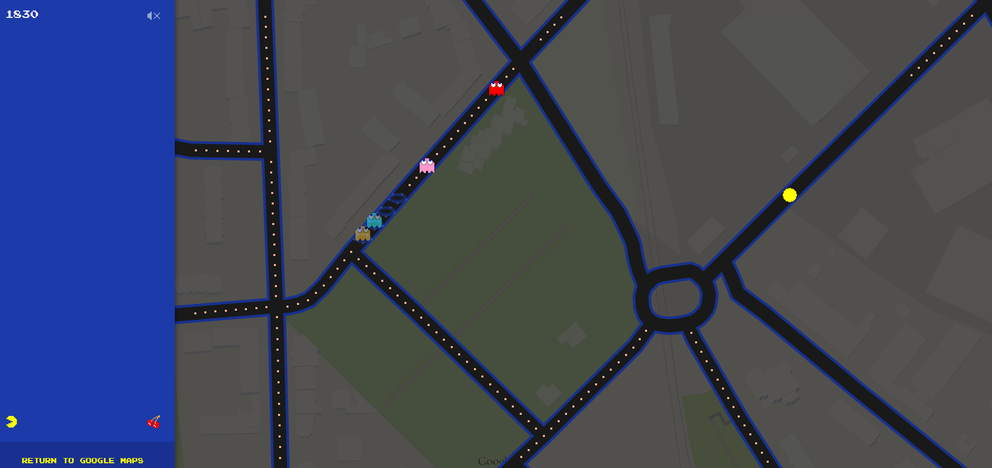
\includegraphics[width=0.9\textwidth]{2-Spielideen/2-3-Related_Work/pacman.png}
     \caption{Pacman auf Googlemaps
	(Quelle: \url{http://media2.giga.de/2015/03/pacman-google-maps-rcm992x0.png})
		}
\end{figure}


\subsubsection{Twinkomplex}

Eine andere Idee hatte der Entwickler von TwinKomplex \footnote{\url{http://twinkomplex.browsergames.de/}}. Er l�sst den Spieler in die Rolle eines Agenten schl�pfen. Dieser wird, mit Hilfe von Google-Maps und Open-Source-Daten, virtuell durch echte Schaupl�tze gef�hrt um F�lle zu l�sen. Hier wird die reale Welt in ein virtuelles Spiel eingearbeitet.

\begin{figure}[htbp]
  \centering
    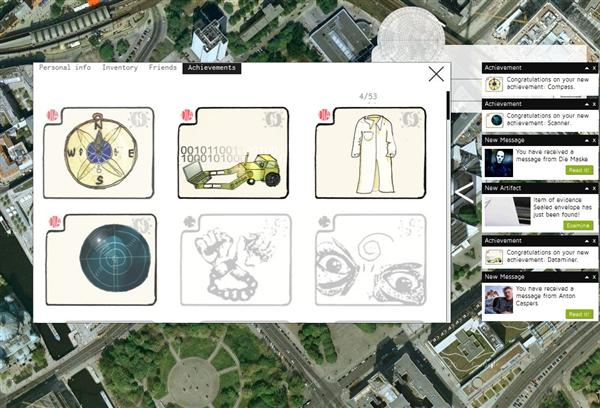
\includegraphics[width=0.65\textwidth]{2-Spielideen/2-3-Related_Work/twinkomplex.png}
     \caption{Screenshot des Spiels TwinKomplex. Auf einer reellen Karte gilt es Dinge zu finden bzw. mit Hilfe von einigen Utensilien einen Fall zu l�sen.
		(Quelle: \url{http://www.onlinegameslist.org/wp-content/uploads/2012/01/twinkomplex-game-achievements.jpg})
		}
\end{figure}

\subsubsection{Geocaching}

%Geocaching wird durch eine stark wachsende Gemeinschaft vertreten. Es gibt bereits �ber 2.630.700 "`Caches"' auf der Welt \footnote{\url{https://www.geocaching.com/play}}.  
Geocaching ist eine Art Schnitzeljagd. Mithilfe von GPS-Daten und Ger�ten, die einem dabei behilflich sein k�nnen (z.B. Smartphone), gilt es von anderen Mitspielern Verstecke (Caches) zu finden. Meist sind in diesen Caches Logb�cher und/oder Tauschgegenst�nde versteckt. Auch R�tsel, die zu einem n�chstes Cache f�hren sind �blich. Oft sind zusammenh�ngende Folgen von Verstecken thematisch gestaltet.
Geocaching hat eine gro�e Community und ist viel mehr auf Engagement der Community-Mitglieder sowie auf direkte und indirekte soziale Interaktion ausgelegt, als die anderen vorgestellten Beispiele \cite{ohara}. 5
�hnlich den erarbeiteten Spielideen werden beim Geocaching GPS-Daten zur Orientierung verwendet.
%Wichtig beim Spielen von Geocaching ist, dass die Menschen, die nicht mit dem Spiel vertraut sind (sogenannte Muggels) nicht sehen d�rfen wie man die Caches hervorholt bzw. versteckt. 


%\begin{figure}[htbp]
 % \centering
  %  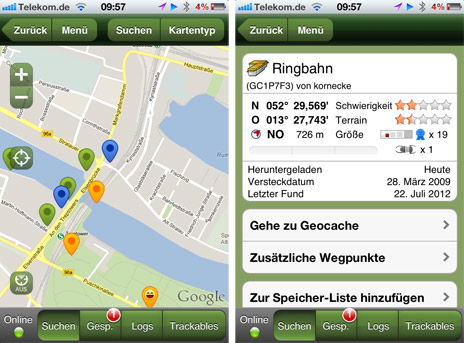
\includegraphics[width=0.65\textwidth]{2-Spielideen/2-3-Related_Work/geocaching-app.png}
   %  \caption{Die Geocaching-App. Auf der Karte werden verschiedene Caches dargestellt. Rechts sieht man Details zu einem ausgew�hlten Cache.
	%	(Quelle: \url{http://www.iphone-ticker.de/wp-content/uploads/2012/08/geocaching-app.jpg})
	%	}
%\end{figure}

\chapter{Spielkonzepte}



Einige Hilfsmittel, die zur Umsetzung der oben genannten Beispiel-Spiele notwendig oder
hilfreich sind.

Um die oben genannten Spiele um einen virtuellen Teil erweitern zu k�nnen werden Konzepte ben�tigt. Eine von uns getroffene Auswahl wird im folgenden beschrieben. 

\section{Erweiterte Realit�t}
Konzepte, die explizit die Realit�t erweitern und dadurch einen Mehrwert zum Spiel beitragen.


\subsubsection{Integration virtueller Objekte in die physische Umgebung}\label{sec:integration-virtueller-objekte-in-die-physische-umgebung}
Um ein virtuelles Spiel in die physische Umgebung integrieren zu k�nnen, m�ssen auch alle Objekte des virtuellen Spieles in die physische Umgebung gebracht werden. Dies kann z.B. auf einer virtuellen Karte, die die Wirklichkeit widerspiegelt, geschehen.

Zum Beispiel die Items bei unserem Spiel Snake, die es einzusammeln gilt, werden auf einer Karte auf dem Smartphone dargestellt und durch einen eingeschr�nkten Zufall platziert. Bei dem ein oder anderen Spiel soll es eine Basis f�r jedes Team geben. Dabei bietet sich an, dieses auf eine relativ freie Fl�che festzusetzen. Generell sollte darauf geachtet werden, dass die Objekte nicht innerhalb eines Geb�udes landen oder in nicht begehbares/erreichbares Terrain platziert werden.



Dies kann mit Hilfe der folgenden technischen L�sungen umgesetzt werden. Die Kartendarstellung (s. \ref{kartendarstellung}) hilft enorm die Objekte in die physische Welt einzuarbeiten, da sie lediglich auf der Karte eingef�gt werden m�ssen. Mit der Kollisionsabfrage (s. \ref{kollisionsabfrage}) kann eine Kollision zweier Objekte, zum Beispiel eine "`Snake"' mit einem "`Item"', verwirklicht werden. Die Positionsabfrage wird unter anderem daf�r ben�tigt um sicherzustellen, dass das Objekt in der N�he des Spielers erstellt wird. (s. \ref{positionsermittlung}).

\subsubsection{Darstellung der physischen und virtuellen Umgebung}\label{sec:darstellung-der-physischen-und-virtuellen-umgebung}

Die physische Welt in eine virtuelle Umgebung zu �bertragen kann einen enormen Mehrwert des Spiels darstellen.
Sei es in einer Karte als �bersicht oder lediglich eine Anzeige ob man sich innerhalb bzw. au�erhalb des Spielfelds befindet. Des weiteren kann mit den heutigen Smartphones auch wie in  Abbildung \ref{fig:aug01} gezeigt eine Augmented Reality geschaffen werden, die die Darstellung der realen Welt um etwa die Beschriftung der zu sehenden Gesch�fte erweitert.
\begin{figure}[htbp]
  \centering
    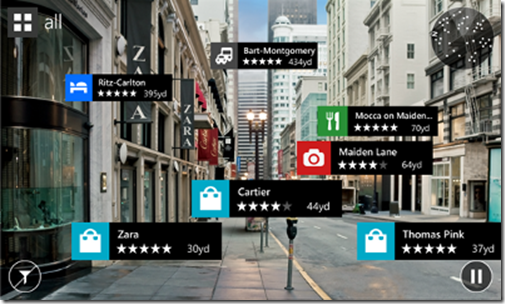
\includegraphics[width=0.9\textwidth]{3-Spielkonzepte/3-1-Erweiterte_Realitaet/map01.png}
    
		\caption{Handyscreen um die zu sehenden Gesch�fte, Hotels, etc. erweitert
	(Quelle: \url{http://blogs.bing.com/maps/wp-content/uploads/sites/3/2013/06/clip_5F00_image006_5F00_thumb_5F00_4AEFDB0C.png})
		}
		\label{fig:aug01} 
\end{figure}
 Hierf�r werden Kartendarstellung (s. \ref{kartendarstellung}) und Positionsermittlung (s. \ref{positionsermittlung}) ben�tigt.

\subsubsection{Kollision virtueller Objekte}\label{sec:kollision-virtueller-objekte}
Treffen zwei virtuelle Objekte aufeinander kann ein Event ausgel�st werden. Wird bei Snake z.B. der eigene Schwanz ber�hrt, was laut der Regeln nicht erlaubt ist, muss dies dem Spieler mitgeteilt werden und evtl. weitere Ereignisse ausgef�hrt werden.

Dazu werden die Kollisionsabfrage (s. \ref{kollisionsabfrage}) und die  Positionsermittlung (s. \ref{positionsermittlung}) gebraucht.


\subsubsection{Einsammeln von Objekten}\label{sec:einsammeln-von-objekten}
Eine Variante der Kollision mit virtuellen Objekten ist das Einsammeln. Wenn ein Spieler in Reichweite eines Items ist, das es einzusammeln gilt, kann dies entweder automatisch passieren oder �ber eine Aufforderung auf dem mobilen Ger�t. Zur Best�tigung, dass etwas eingesammelt wurde, kann nun wiederum ein akustisches oder haptisches Signal gegeben werden.

 Erreicht werden kann dies durch die Positionsermittlung (s. \ref{positionsermittlung}) und die Kollisionsabfrage (s. \ref{kollisionsabfrage}). F�r weitere Best�tigungssignale sind auch andere Sensorik (s. \ref{sensorik}) von Vorteil.


\section{Benutzer Interface}



Konzepte, die haupts�chlich dazu dienen mit dem Spieler zu interagieren und sehr abh�ngig von seinen Entscheidungen sind.


\subsubsection{Kompass}
\begin{wrapfigure}{r}{0.4\textwidth}
  \begin{center}
    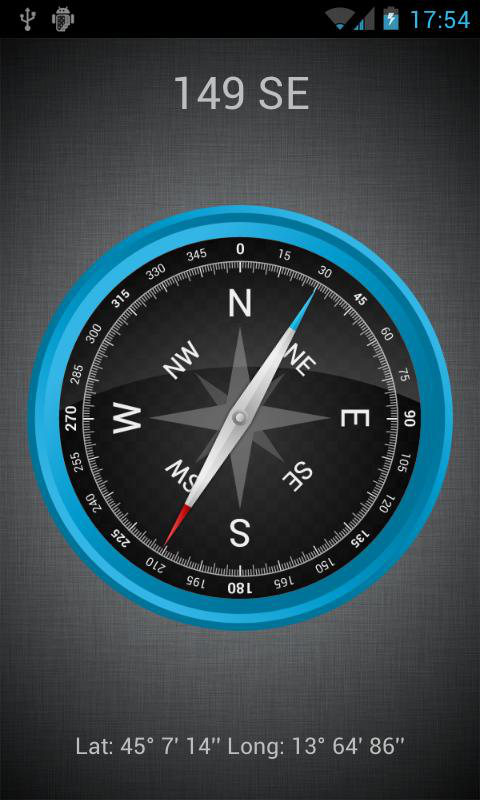
\includegraphics[width=0.3\textwidth]{3-Spielkonzepte/3-2-Benutzer_Interface/kompass.png}
     \caption{integrierter Kompass unter Android}
  \end{center}
\end{wrapfigure}

Eine Richtungsangabe kann eine Karte ersetzen. Sei es um bei �Capture the Flag� die
Richtung der Fahne des Gegners anzuzeigen oder f�r die �Snake� das n�chste
einzusammelnde Item. In der Regel hat es hier weniger Sinn, wenn die Kompassnadel nach
Norden zeigt.
\newline
Technische L�sungen:
Positionsermittlung (s. \ref{positionsermittlung}), GUI (s. \ref{gui}), Andere Sensorik (s. \ref{sensorik})

\subsubsection{Akustische und haptische Orientierungshilfen}

Akustische oder haptische Signale k�nnen ebenso Hinweise geben auf in der N�he
befindliche Interessengebiete (z.B. ert�nen eines Signals oder Vibration bei erreichen eines
bestimmtem Umkreises von einem Item). 
K�nnen aber auch als Best�tigung eingesetzt
werden, wenn z.B. etwas eingesammelt wurde.
\newline
Technische L�sungen:
Kollisionsabfrage (s. \ref{kollisionsabfrage}), Andere Sensorik (s. \ref{sensorik})


\subsubsection{Geschwindigkeitsmessung}
Um das Spielgeschehen besser zu kontrollieren zu k�nnen, kann eine Messung der
Geschwindigkeit von Vorteil sein. M�chten wir z.B. bei Capute the Flag dem Fahnentr�ger
nicht erlauben eine gewissen Geschwindigkeit zu �berschreiten, ist eine
Geschwindigkeitsmessung unabdingbar.
\newline
Technische L�sungen:
Positionsermittlung (s. \ref{positionsermittlung}), Server-Client-Kommunikation (s. \ref{kommunikation}), Andere Sensorik (s. \ref{sensorik})


\subsubsection{Mensch-Maschine-Kommunikation}
Das komplette Spielgeschehen lebt nach der Integrierung von mobilen Endger�ten von der Kommunikation zwischen Mensch und Ger�t. Wird auf dem Endger�t ein Kompass angezeigt, muss der Spieler insofern reagieren, dass er sich in die richtige Richtung dreht.
Wenn er etwas einsammeln m�chte, kann es erforderlich sein, dass ein Button gedr�ckt
wird.
\newline
Technische L�sungen:
GUI (s. \ref{gui}), Kartendarstellung (s. \ref{kartendarstellung})

\section{Kompass}

Eine Richtungsangabe kann eine Karte ersetzen. Sei es um bei �Capture the Flag� die
Richtung der Fahne des Gegners anzuzeigen oder f�r die �Snake� das n�chste
einzusammelnde Item. In der Regel hat es hier weniger Sinn, wenn die Kompassnadel nach
Norden zeigt.
\newline
Technische L�sungen:
Positionsermittlung (s. \ref{positionsermittlung}), GUI (s. \ref{gui}), Andere Sensorik (s. \ref{sensorik})

/% \section{Arkustische und haptische Orientierungshilfen}

Akustische oder haptische Signale k�nnen ebenso Hinweise geben auf in der N�he
befindliche Interessengebiete (z.B. ert�nen eines Signals oder Vibration bei erreichen eines
bestimmtem Umkreises von einem Item). K�nnen aber auch als Best�tigung eingesetzt
werden, wenn z.B. etwas eingesammelt wurde.
\newline
Technische L�sungen:
Kollisionsabfrage (s. \ref{kollisionsabfrage}), Andere Sensorik (s. \ref{sensorik})

/% \section{Synchronisation zwischen mobilen Endger�ten}

Und hier wieder einf�gen.

/% \section{Kollision virtueller Objekte}
Treffen zwei virtuelle Objekte aufeinander muss in der Regel ein Event ausgel�st werden.
Wird bei Snake z.B. der eigene Schwanz ber�hrt, was laut der Regeln nicht erlaubt ist, muss
dies dem Spieler mitgeteilt werden und evtl. weitere Ereignisse ausgef�hrt werden.
\newline
Technische L�sungen:
Kollisionsabfrage (s. \ref{kollisionsabfrage}), Positionsermittlung (s. \ref{positionsermittlung})

/% \section{Einsammeln von Objekten}
Eine Variante der Kollision mit virtuellen Objekten ist das Einsammeln. Wenn ein Spieler in
Reichweite eines Items ist, das es einzusammeln gilt, kann dies entweder automatisch
passieren oder �ber eine Aufforderung auf dem mobilen Ger�t. Zur Best�tigung, dass
etwas eingesammelt wurde, kann nun wiederum ein akustisches oder haptisches Signal
gegeben werden.

/% \section{Geschwindigkeitsmessung}
Um das Spielgeschehen besser zu kontrollieren zu k�nnen, kann eine Messung der
Geschwindigkeit von Vorteil sein. M�chten wir z.B. bei Capute the Flag dem Fahnentr�ger
nicht erlauben eine gewissen Geschwindigkeit zu �berschreiten, ist eine
Geschwindigkeitsmessung unabdingbar.
\newline
Technische L�sungen:
{\color{red}add Links zu}
Positionsermittlung, Server-Client-Kommunikation, Andere Sensorik

/% \section{Mensch-Maschine-Kommunikation}
Das komplette Spielgeschehen lebt nach der Integrierung von mobilen Endger�ten von der Kommunikation zwischen Mensch und Ger�t. Wird auf dem Endger�t ein Kompass angezeigt, muss der Spieler insofern reagieren, dass er sich in die richtige Richtung dreht.
Wenn er etwas einsammeln m�chte, kann es erforderlich sein, dass ein Button gedr�ckt
wird.
\newline
Technische L�sungen:
GUI (s. \ref{gui}), Kartendarstellung (s. \ref{kartendarstellung}), Andere Sensorik (s. \ref{sensorik})

/% \section{Chat}
Um mit seinen Teammitgliedern oder dem gegnerischen Team zu kommunizieren gibt es
eine Reihe von M�glichkeiten. Wenn man sich au�er Sicht- und H�rweite befindet kann
dies �ber ein mobiles Ger�t stattfinden. Beim Chat wird eine Nachricht verschickt, die der
Empf�nger auf seinem Ger�t einsehen kann und dann seinerseits eine Antwort verfassen
kann.
\newpage
\chapter{Technische L�sungen}
\label{technisch}
\section{Positionsermittlung}

\subsection{LocationManager vs LocationClient}

Im folgenden werden zwei m�gliche Dienste zur Positionsermittlung verwendet. Der LocationManager\footnote{{\url{http://developer.android.com/reference/android/location/LocationManager.html}}} und der LocationClient\footnote{{\url{http://www.doc.ic.ac.uk/project/2013/271/g1327125/android-studio/sdk/extras/google/google_play_services/docs/reference/com/google/android/gms/location/LocationClient.html}}}.


\subsubsection{LocationManager}

Der LocationManager ist ein von Android bereitgestellter Dienst, der �ber den GPS Sensor die Position des Smartphones ermittelt.
Ein Vorteil bei verwendenden dieses Dienstes ist, das man nicht an die Dienste von Google gebunden ist, und somit theoretisch auch f�r
nicht Google-Konforme Androidbetriebssysteme entwickeln kann. Da nur der GPS Sensor verwendet wird, w�re eine entsprechende Anwendung sogar unabh�ngig von einer Internetverbindung. Auch wird dieser Dienst auch noch von �lteren Android Versionen unterst�tzt.
Nachteilig wird in einer Forendiskussion \footnote{http://stackoverflow.com/questions/20908822/android-difference-between-locationmanager-addproximityalert-locationclien {\color{red}}bessere Quelle} der hohe Akku verbrauch genannt.


\subsubsection{LocationClient}

Der LocationClient ist ein von Google bereitgestellter Dienst, der �ber den GPS Sensor und andere Quellen, die Google zur Verf�gung stellt, die Position des Smartphones zu ermitteln. Als Vorteile dieses Dienstes werden in der oben schon erw�hnten Forendiskussion wird erw�hnt, dass dieser Dienst Akku-schonender sei. Auch sei er zuverl�ssiger. Die anderen Quellen zur Positionsermittlung k�nnten auch zu einer genauen Positionsermittlung beitragen, wenn es eventuell �bertragungsprobleme zum GPS-Satelliten gibt.
Nachteilig an diesem Dienst ist, dass man eine Internetverbindung ben�tigt. Au�erdem werden die Google Play Services vorausgesetzt, welche erst ab Android Version 2.2 zur Verf�gung stehen. Zudem ist man von Google abh�ngig.


\subsubsection{Messdaten}

Um LocationManager und LocationClient f�r unsere Zwecke vergleichen zu k�nnen, wurde ein Testprogramm entwickelt, welches jeweils in zwei separaten Activities GPS Messdaten in einer Datei sammelt. Es werden jeweils Koordinaten und Genauigkeit gesammelt. Zur optischen Darstellung der Ergebnisse wird aus den aufgezeichneten Koordinate eine Linie (PolyLine\footnote{{\url{https://developer.android.com/reference/com/google/android/gms/maps/model/Polyline.html}}) gezeichnet. Als Vergleich wird eine Luftlinie zwischen Anfangs- und Endpunkt gezogen. \newline
Im Folgenden werden nun die ausgewerteten Sensordaten dargestellt.

\begin{table}[h]
\caption{Location Versuch 1}
\begin{tabular}{l|l|l|}
\cline{2-3}
                                      & locationClient         & locationManager         \\ \hline
\multicolumn{1}{|l|}{Datum}           & \multicolumn{2}{l|}{10.12.2014}                  \\ \hline
\multicolumn{1}{|l|}{Ort}             & \multicolumn{2}{l|}{Universit�t Koblenz, Campus} \\ \hline
\multicolumn{1}{|l|}{Wetter}          & \multicolumn{2}{l|}{Bew�lk, leichter Niesel}     \\ \hline
\multicolumn{1}{|l|}{Ger�t}           & \multicolumn{2}{l|}{Samsung Galaxy S3}           \\ \hline
\multicolumn{1}{|l|}{Genauigkeit}     & 7,049                  & 8,698                   \\ \hline
\multicolumn{1}{|l|}{Updates/Sekunde} & 0,936                  & 1,016                   \\ \hline
\end{tabular}
\label{tab:lV1}
\end{table}

\begin{table}[h]
\caption{Location Versuch 2}
\begin{tabular}{l|l|l|}
\cline{2-3}
                                      & locationClient                & locationManager                \\ \hline
\multicolumn{1}{|l|}{Datum}           & \multicolumn{2}{l|}{14.12.2014}                                \\ \hline
\multicolumn{1}{|l|}{Ort}             & \multicolumn{2}{l|}{Ransbach-Baumbach, L307richtung Mogendorf} \\ \hline
\multicolumn{1}{|l|}{Wetter}          & \multicolumn{2}{l|}{Wetter:,leicht bew�lk leicht windig}       \\ \hline
\multicolumn{1}{|l|}{Ger�t}           & \multicolumn{2}{l|}{Samsung Galaxy S3}                         \\ \hline
\multicolumn{1}{|l|}{Genauigkeit}     & 5,482                         & 6,216                          \\ \hline
\multicolumn{1}{|l|}{Updates/Sekunde} & 1,003                         & 0,969                          \\ \hline
\end{tabular}
\label{tab:lV2}
\end{table}

Hierbei muss noch erg�nzt werden, dass der Genauigkeitswert folgenderma�en beschrieben wird. An L�ngen- und Breitengrad
der Position wird ein Kreis mit Radius der Genauigkeit gezeichnet. Es besteht eine 68-prozentige Wahrscheinlichkeit, dass
sich die Position innerhalb des Kreises Befindet\footnote{http://developer.android.com/reference/android/location/Location.html}.
Es gilt, je kleiner der Wert desto besser. In den Tabellen wurde jeweils das arithmetische Mittel der aufgezeichneten Genauigkeiten eingetragen.



\subsection{Genauigkeit}
Nun folgen eine grafische Darstellung der Genauigkeitsaufzeinungen die mit dem Testprogramm gemacht wurden

  \begin{figure}[h]
    \begin{center}
    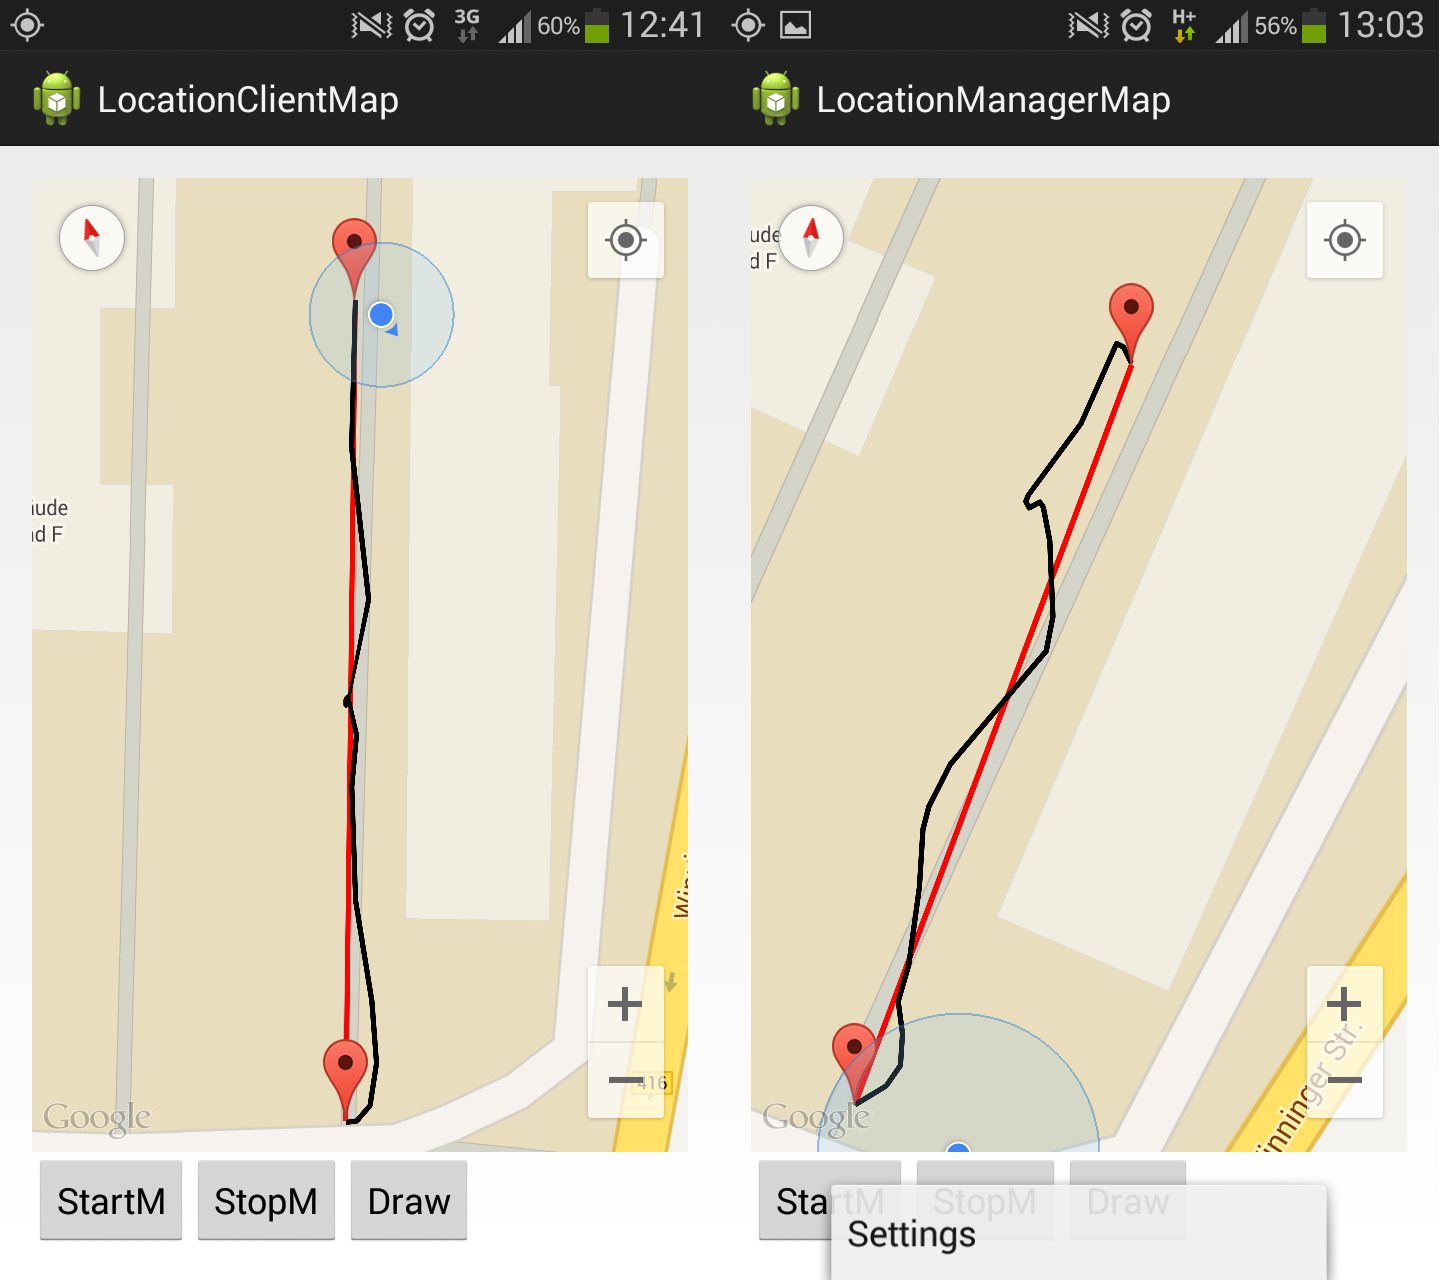
\includegraphics[width=0.48\textwidth]{4-Technische_Loesungen/4-1-Positionsermittlung/Data/Screenshot_2014-12-10-12-41-12_fuusion.png}
    \end{center}
     \caption{Location Versuch 1}
     \label{fig: picLV1}
  \end{figure}

  \begin{figure}[h]
    \begin{center}
    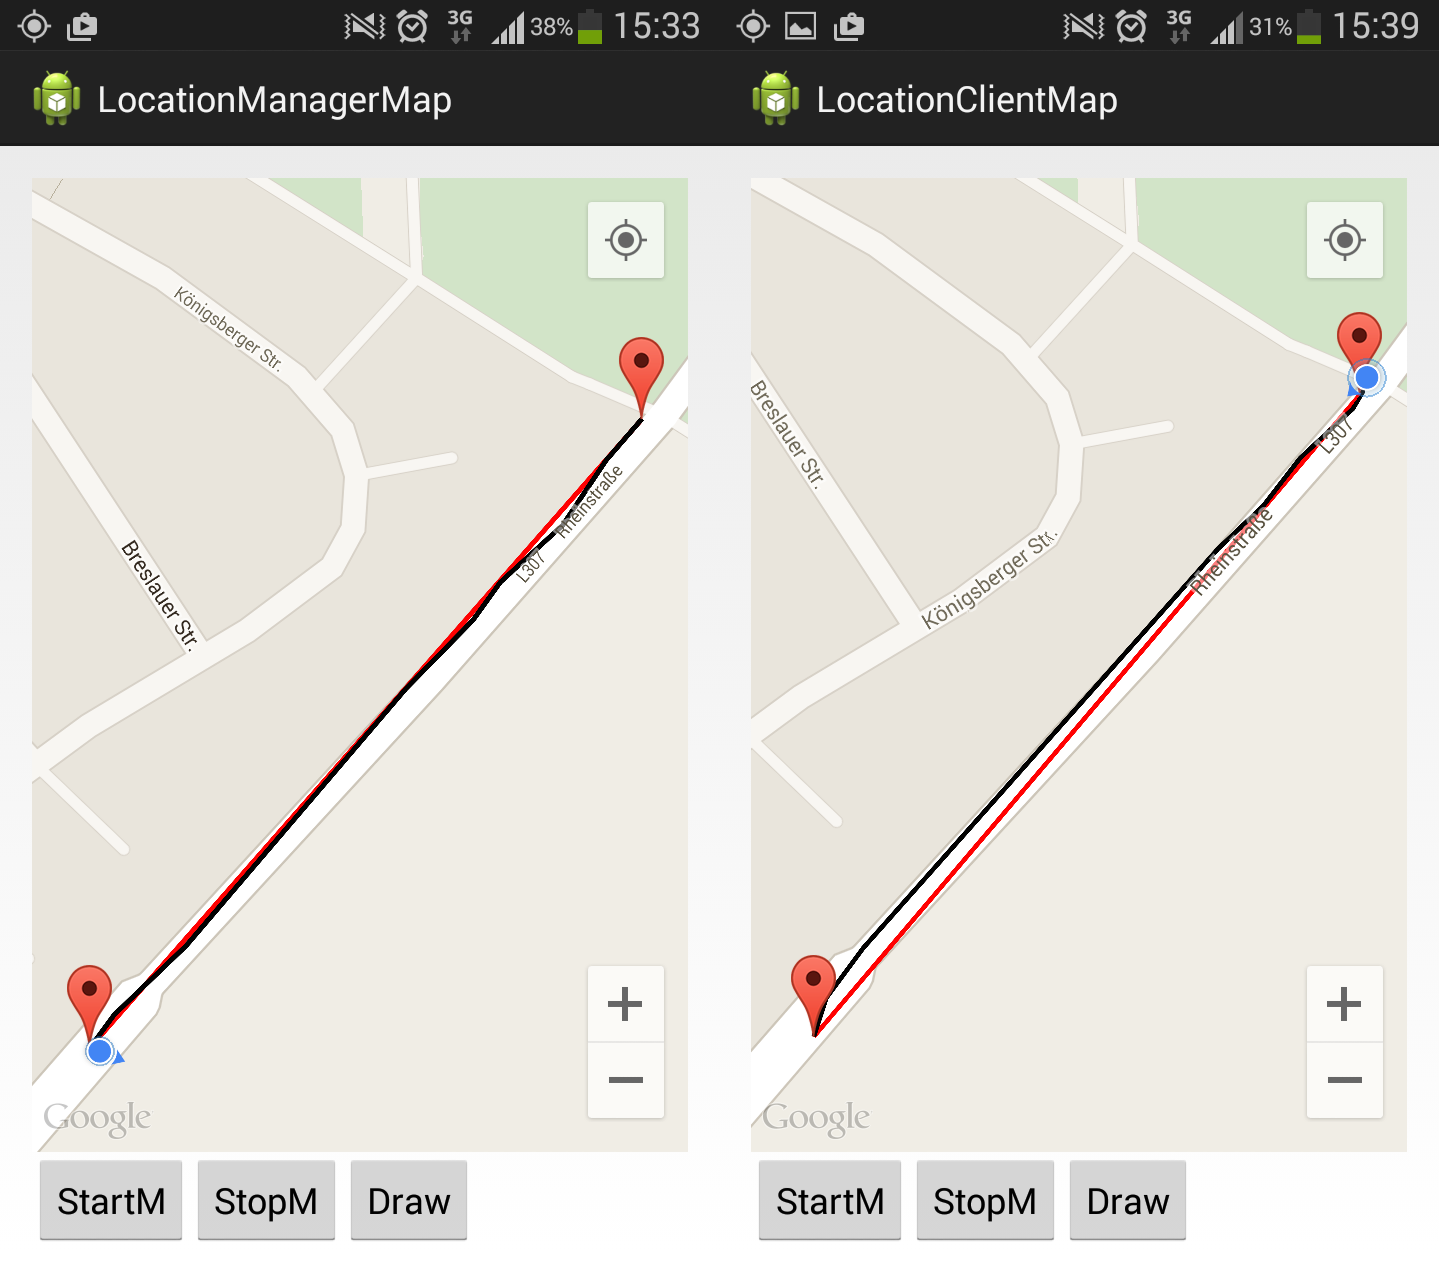
\includegraphics[width=0.48\textwidth]{4-Technische_Loesungen/4-1-Positionsermittlung/Data/Screenshot_2014-12-14-15-33-10_fuusion.png}
     \end{center}
     \caption{Location Versuch 2}
     \label{fig: picLV2}
  \end{figure}
  
  \begin{figure}[h]
    \begin{center}
    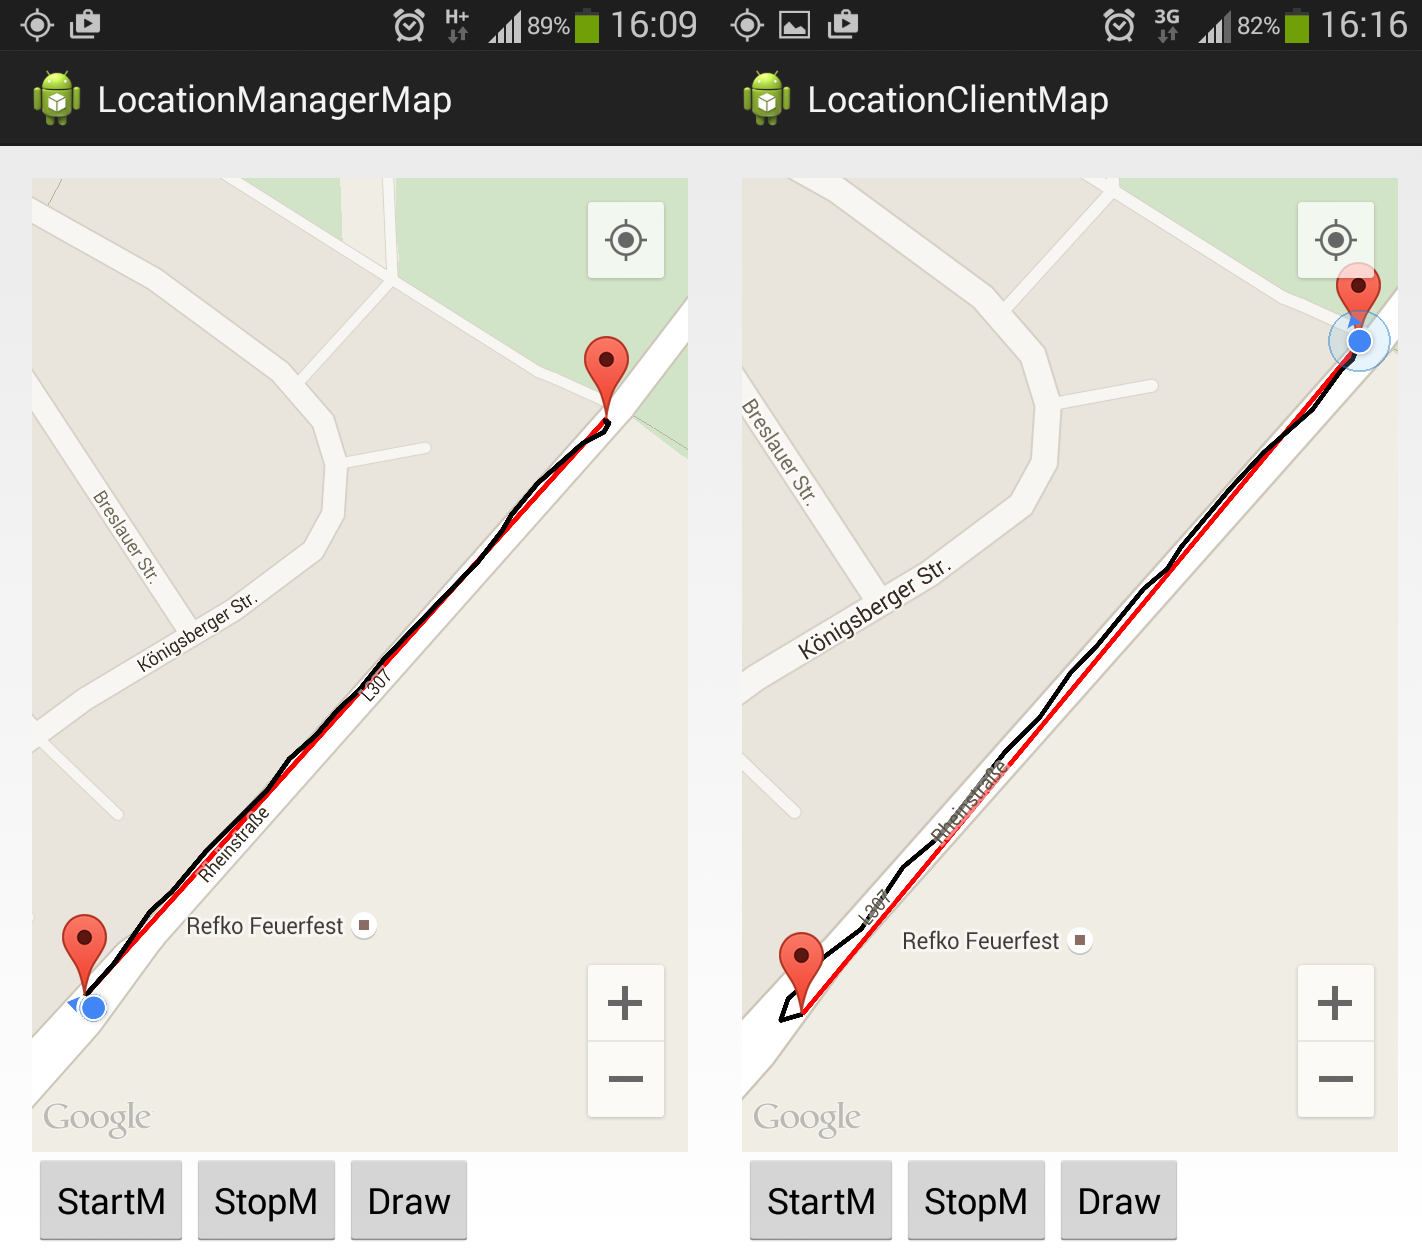
\includegraphics[width=0.48\textwidth]{4-Technische_Loesungen/4-1-Positionsermittlung/Data/Screenshot_2015-05-08-16-09-35_fuusion.png}
     \end{center}
     \caption{Location Versuch 3}
     \label{fig: picLV3}
  \end{figure}
	
	\begin{figure}[h]
    \begin{center}
    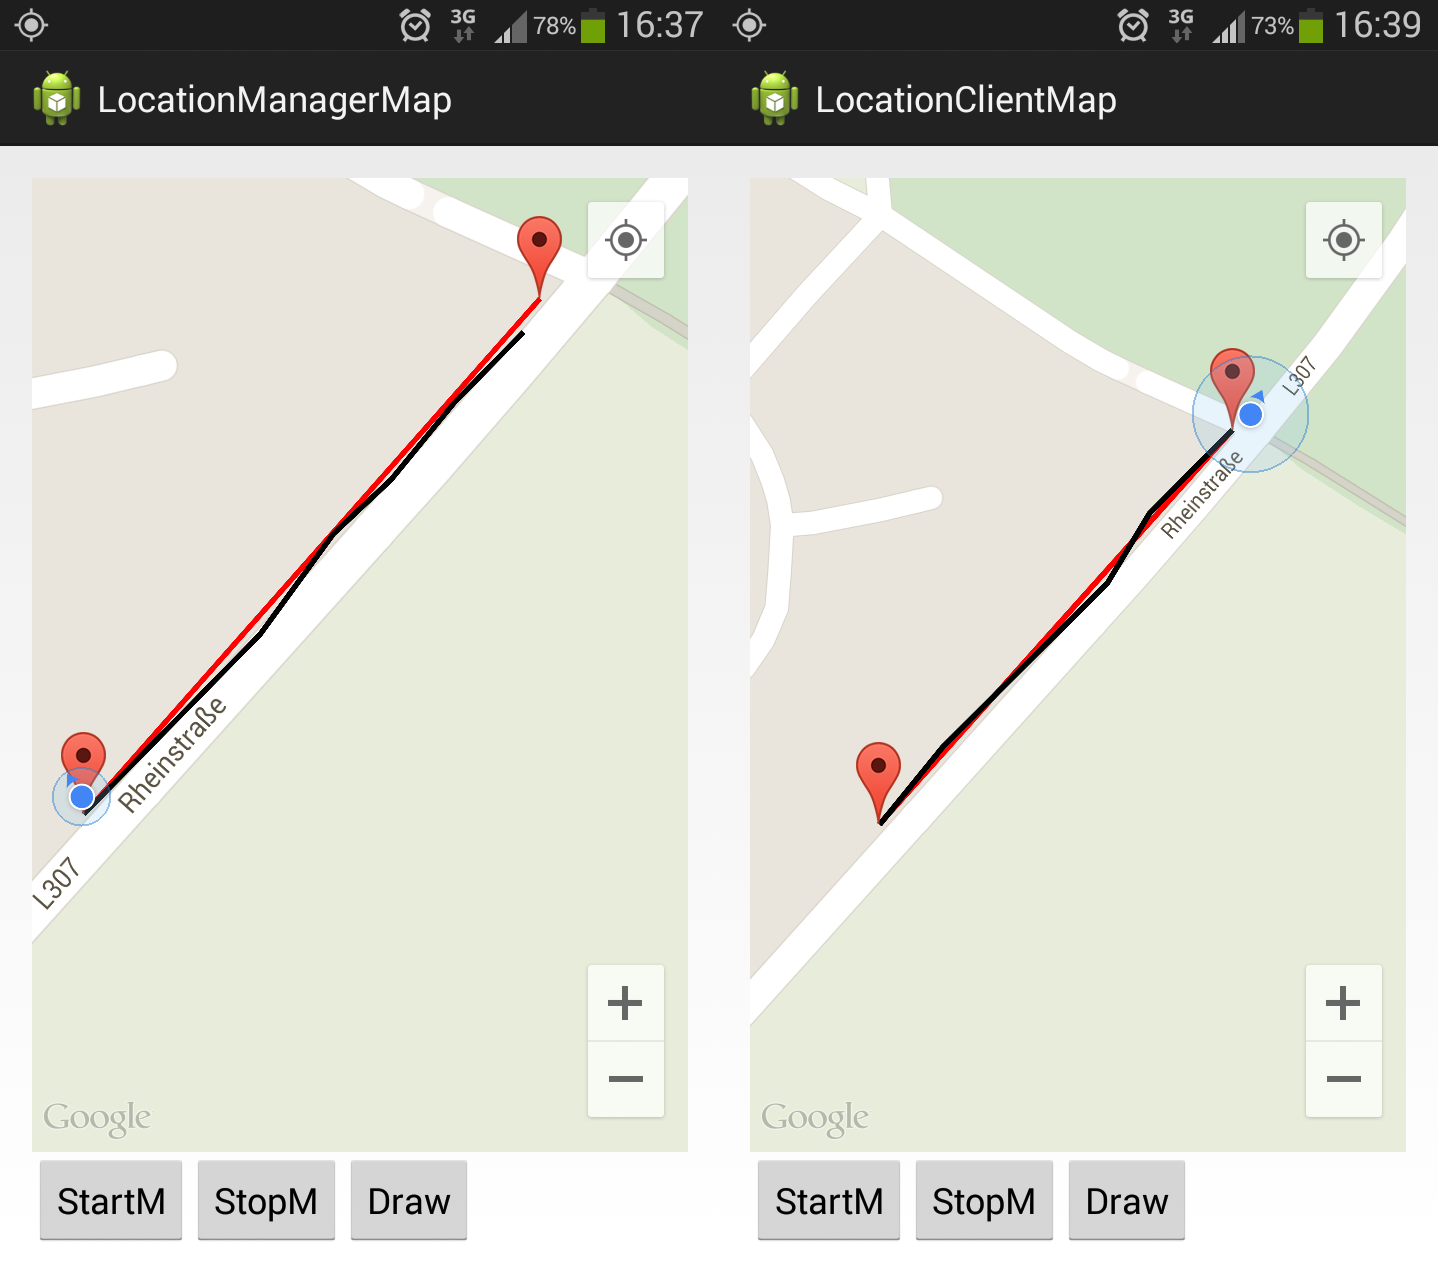
\includegraphics[width=0.48\textwidth]{4-Technische_Loesungen/4-1-Positionsermittlung/Data/Screenshot_2015-05-08-16-37-21_fuusion.png}
     \end{center}
     \caption{Location Versuch 4}
     \label{fig: picLV4}
  \end{figure}
	
	\begin{figure}[h]
    \begin{center}
    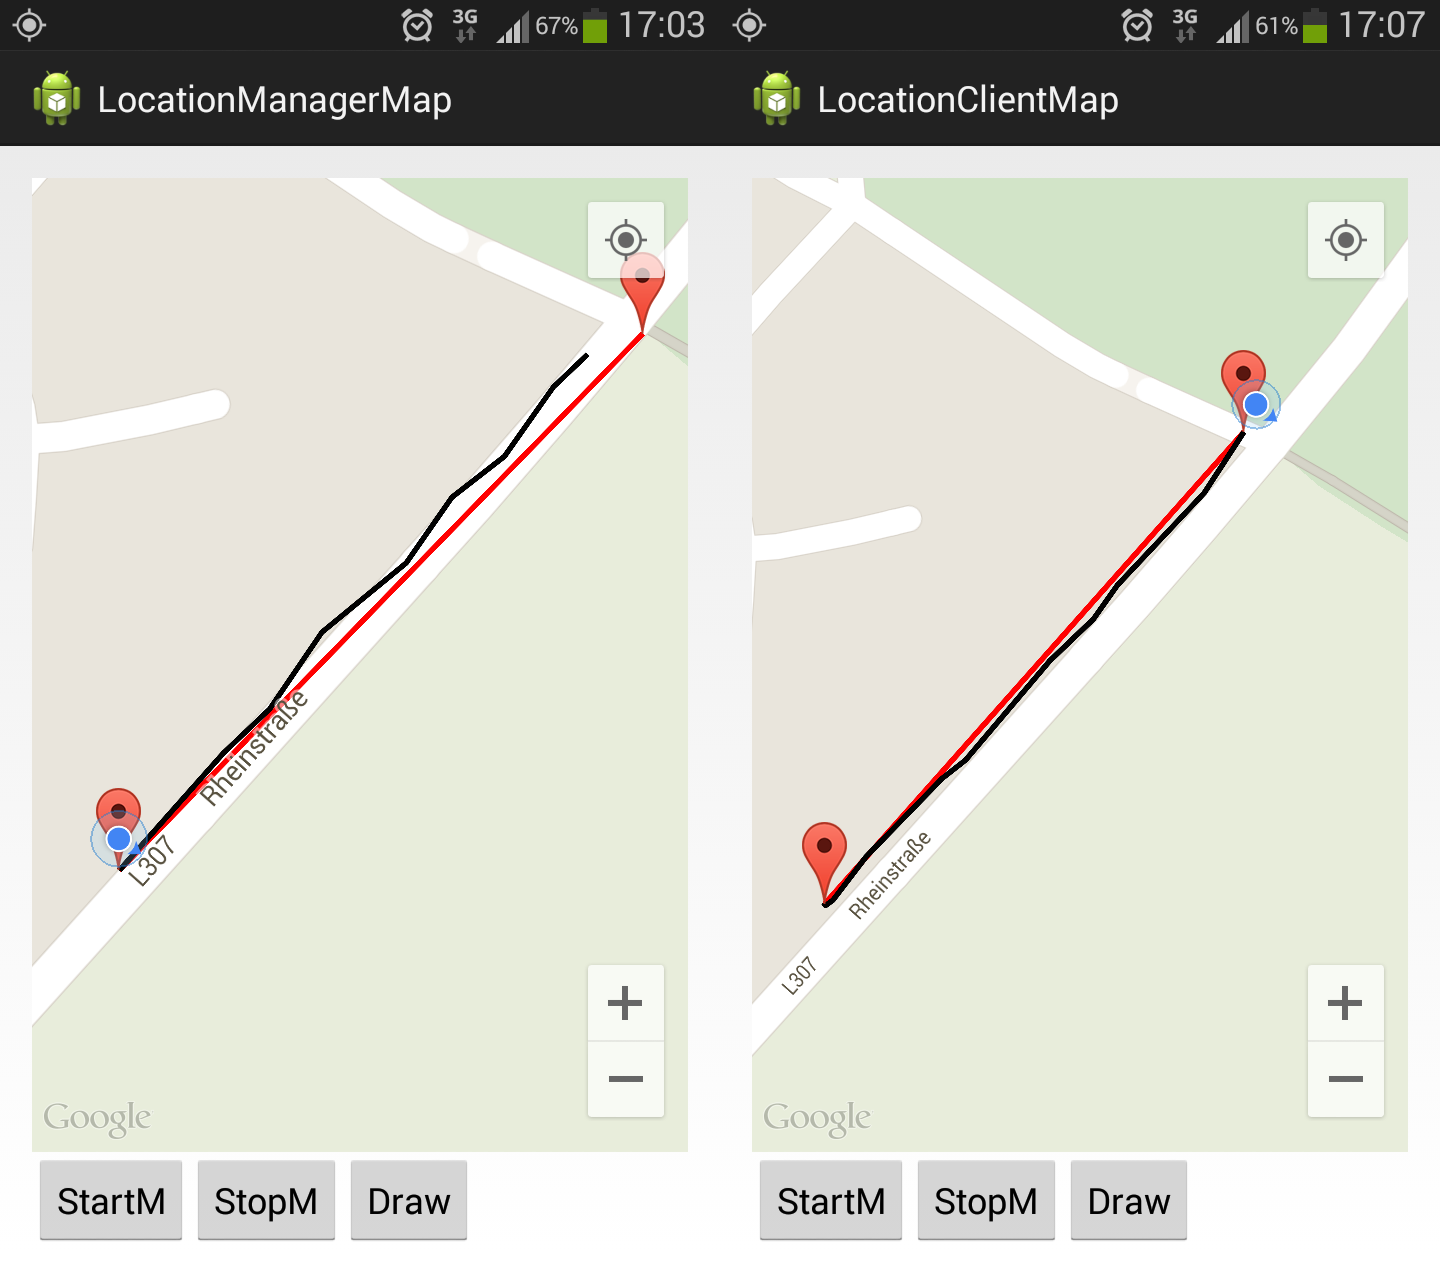
\includegraphics[width=0.48\textwidth]{4-Technische_Loesungen/4-1-Positionsermittlung/Data/Screenshot_2015-05-08-17-03-10_fuusion.png}
     \end{center}
     \caption{Location Versuch 5}
     \label{fig: picLV5}
  \end{figure}
  
  \begin{figure}[h]
    \begin{center}
    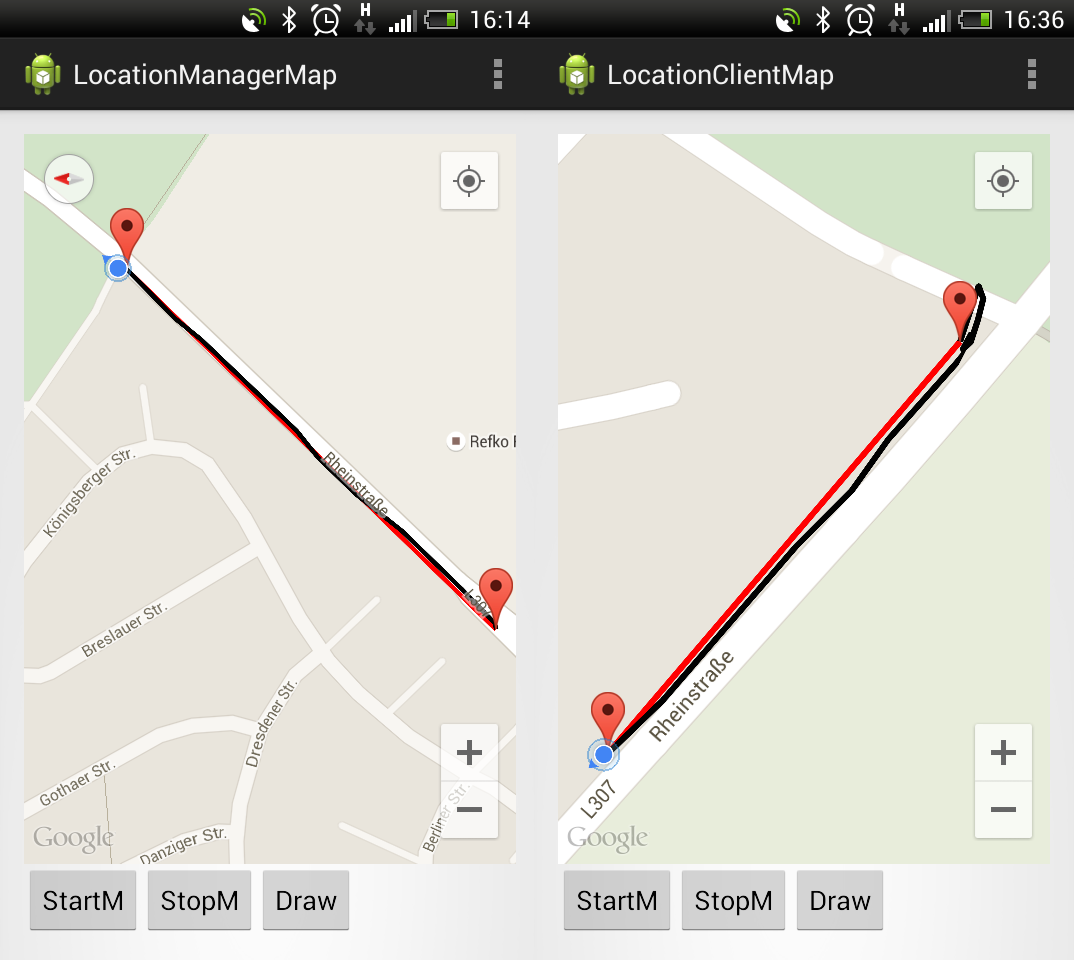
\includegraphics[width=0.48\textwidth]{4-Technische_Loesungen/4-1-Positionsermittlung/Data/2015-05-08_16-14-46_fuusion.png}
     \end{center}
     \caption{Location Versuch 6}
     \label{fig: picLV6}
  \end{figure}
  
  \begin{figure}[h]
    \begin{center}
    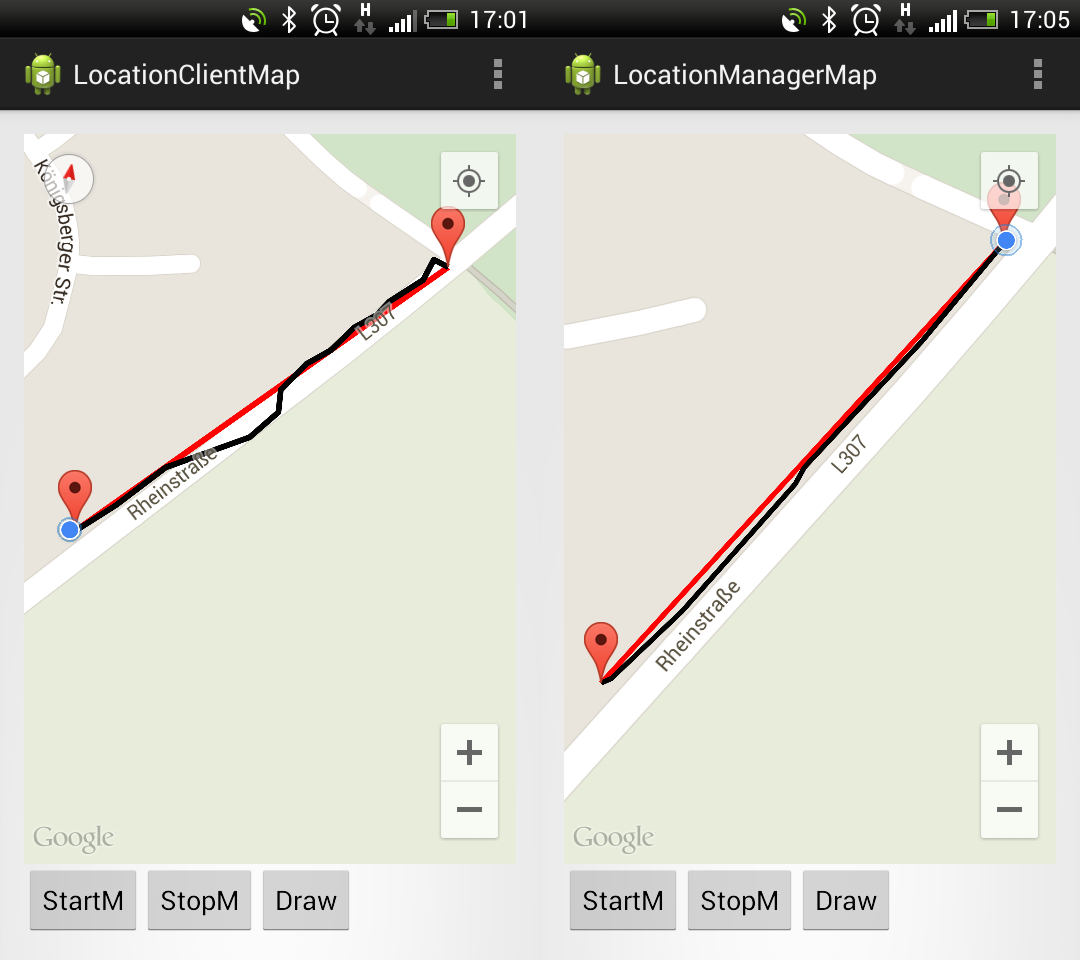
\includegraphics[width=0.48\textwidth]{4-Technische_Loesungen/4-1-Positionsermittlung/Data/2015-05-08_17-01-38_fuusion.png}
     \end{center}
     \caption{Location Versuch 7}
     \label{fig: picLV7}
  \end{figure}
  
  \begin{figure}[h]
    \begin{center}
    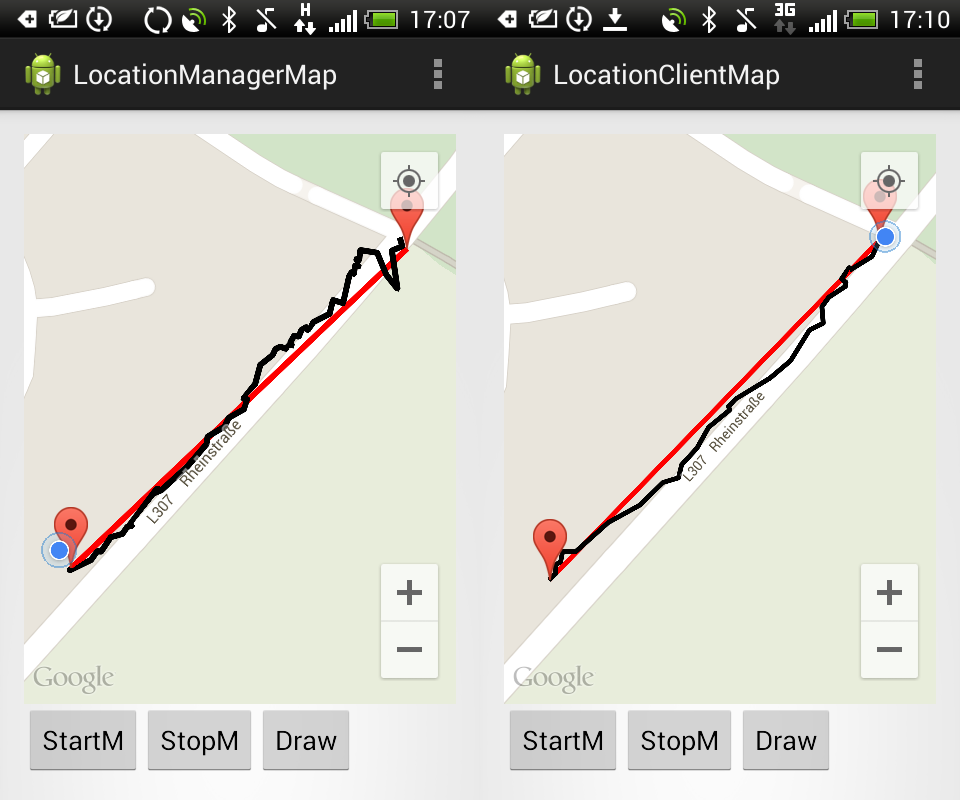
\includegraphics[width=0.48\textwidth]{4-Technische_Loesungen/4-1-Positionsermittlung/Data/Screenshot_2015-05-08-17-07-04_fuusion.png}
     \end{center}
     \caption{Location Versuch 8}
     \label{fig: picLV8}
  \end{figure}
  
  \begin{figure}[h]
    \begin{center}
    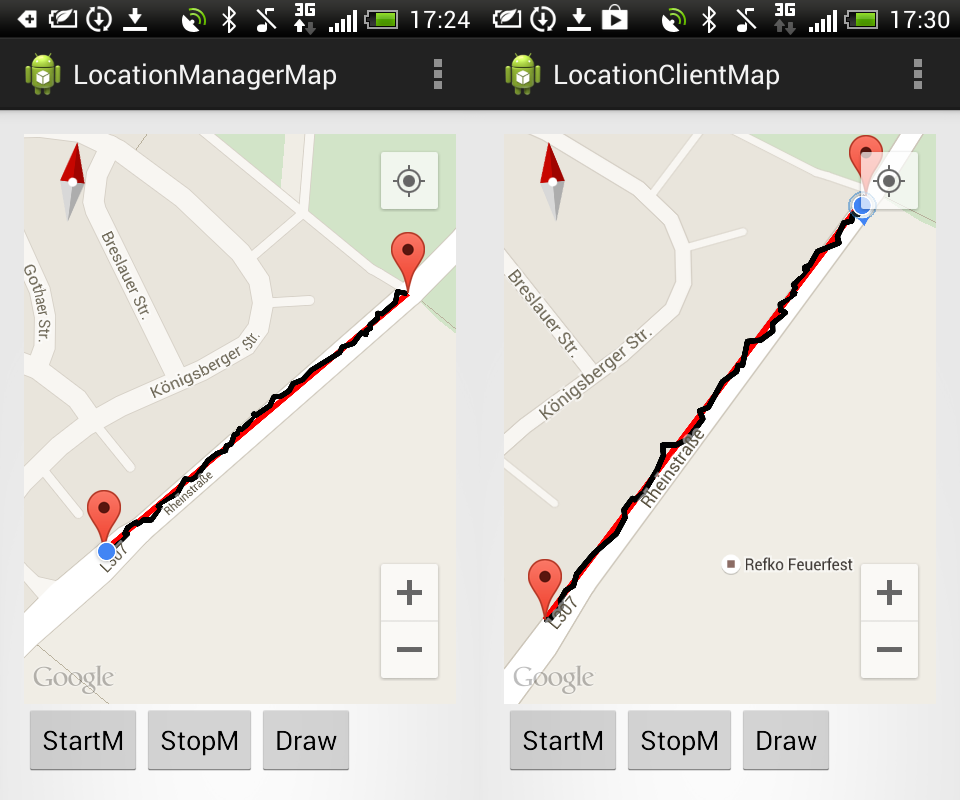
\includegraphics[width=0.48\textwidth]{4-Technische_Loesungen/4-1-Positionsermittlung/Data/Screenshot_2015-05-08-17-24-35_fuusion.png}
     \end{center}
     \caption{Location Versuch 9}
     \label{fig: picLV9}
  \end{figure}
  
  \begin{figure}[h]
    \begin{center}
    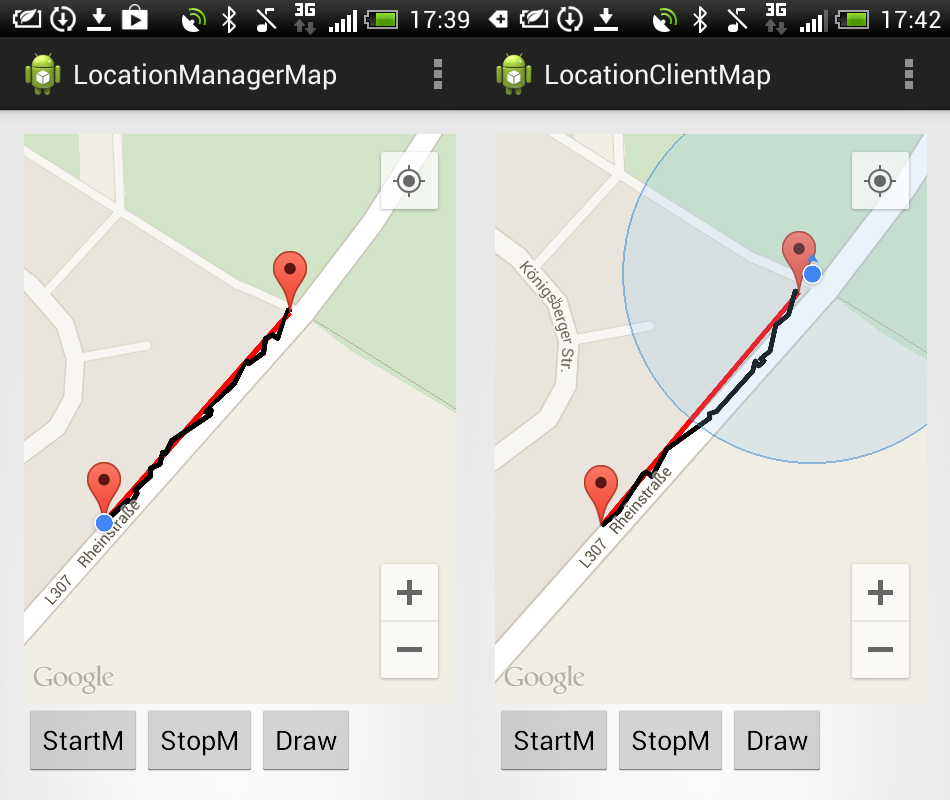
\includegraphics[width=0.48\textwidth]{4-Technische_Loesungen/4-1-Positionsermittlung/Data/Screenshot_2015-05-08-17-39-18_fuusion.png}
     \end{center}
     \caption{Location Versuch 10}
     \label{fig: picLV10}
  \end{figure}
  
  \begin{figure}[h]
    \begin{center}
    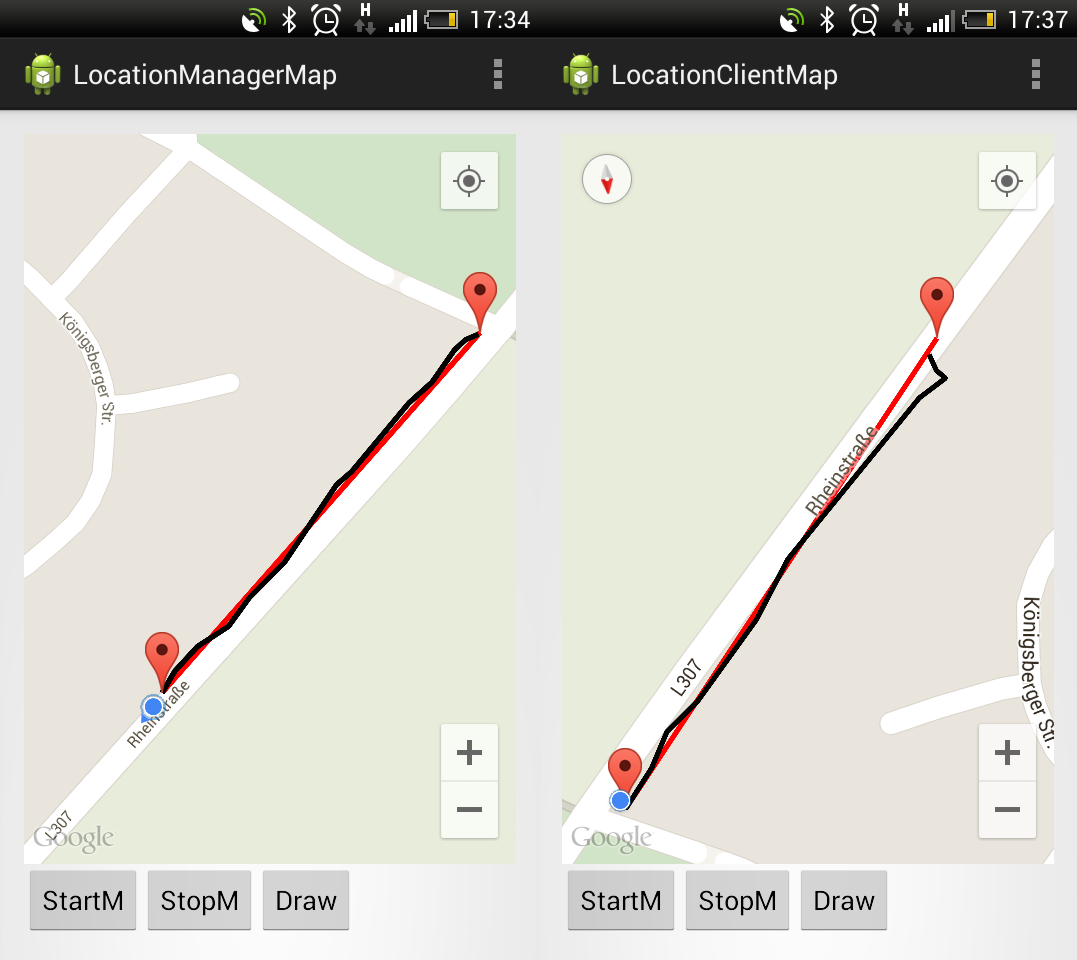
\includegraphics[width=0.48\textwidth]{4-Technische_Loesungen/4-1-Positionsermittlung/Data/2015-05-08_17-34-52_fuusion.png}
     \end{center}
     \caption{Location Versuch 11}
     \label{fig: picLV11}
  \end{figure}
  
\clearpage

\subsection{Fazit}
Die Messdaten belegen, dass der LocationClient minimal die besseren Ergebnisse liefert. Dies ist der Fall bei der Genauigkeit der
Sensordaten und auch bei der grafischen Darstellung. Zweiteres ist ein wichtiger Faktor beim Umsetzten des Snakespiels. Die Unterschiede bei Updates pro Sekunde sind verschwindend gering. Ein weiteres Faktor ist, dass sich schon bereits f�r die Kartenanzeige f�r GoogleMaps entschieden wurde. Da der LocationClient minimal die besseren Ergebnisse liefert und schon ein Dienst von Google verwendet wird, wird zur Positionsermittlung in diesem Projekt der LocationClient verwendet.
\newpage


\section{Kollisionsabfrage}\label{kollisionsabfrage}

S�mtliche Objekte in der Implementation (Spieler, virtuelle Objekte) liegen jeweils nur als Geopositionen (Breiten- und L�ngengrad) vor. Dass zwei Objekte auf dem gleichen Breiten- und L�ngengrad sind ist extrem unwahrscheinlich, da Breiten- und L�ngengrad auf sechs Nachkommastellen genau ist. In der Implementation werden Kollisionen ben�tigt, damit Spieler z.B. in der Lage sind virtuelle Objekte einzusammeln oder eine Kollision zwischen zwei Spieler (Snakespiel) zu realisieren. Im folgenden werden zwei Herangehensweisen vorgestellt.
\subsection*{Kollisionsabfrage �ber Abstandsmessung}\label{abstandsmessung}
%Jedes Spiel verwendet unterschiedliche virtuelle und tats�chliche Objekte. Diese werden zur Kollisionsabfrage in mehrere Kategorien eingeteilt.
%Objekte sind entweder beweglich oder unbeweglich und entweder solide oder unsolide.
%Bei der Kollisionsabfrage k�nnen solide Objekte die passive Rolle und bewegliche Objekte die aktive Rolle einnehmen. 
%Solide bewegliche Objekte k�nnen je nach Situation entweder aktiv oder passiv sein und unter Umst�nden auch mit sich selber kollidieren.
%Jedes bewegliche Objekt nimmt, nachdem seine Positionsdaten ge�ndert wurden, die Rolle des aktiven Objekts ein. Das aktive Objekt wird dann mit jedem soliden Objekt verglichen, das dann die Rolle des passiven Objekts annimmt. Im Falle einer Kollision wird abh�ngig von den beteiligten Objekten ein entsprechender Effekt ausgel�st.
%
%Die meisten Objekte haben Hitboxen in Form eines Kreises.
%Die Android API stellt eine Methode zur Verf�gung, die die Entfernung zwischen zwei Punkten, die �ber geographische Koordinaten bestimmt sind, berechnet \footnote{\url{http://developer.android.com/reference/android/location/Location.html}}. Damit kann die Kollisionsabfrage �ber Abstandsmessung implementiert werden.
%Es wird eine Kollision ausgel�st, falls beide Objekte Kreise sind und die Entfernung zwischen ihren Kreismittelpunkten kleiner ist, als die Summe der Radien.
%
%$|M_{aktiv}-M_{passiv}|<r_{aktiv}+r_{passiv}$
%
%
%Beim Snake-Spiel m�ssen hingegen vier F�lle unterscheiden werden: sowohl das aktive, wie auch das passive beteiligte Objekt k�nnen jeweils einen Kreis oder einen Kette von Kreisen (eine Schlange) als Hitbox haben. Die Schlange wird als Polygonzug von Punkten realisiert. Jeder Eckpunkt ist dabei der Mittelpunkt einer kreisf�rmigen Hitbox (Glied). Die Strecke zwischen zwei aufeinanderfolgenden Eckpunkten des Polygonzuges ist dabei ein Segment der Schlange.
%Das aktive Objekt ist bei Snake immer ein Spieler, also eine Schlange.
%Das passive Objekt kann ein aufsammelbares Bonus-Objekt, ein anderer Spieler oder der aktive Spieler selber sein.
%Das aktive Objekt ist ein Polygonzug, trotzdem m�ssen nur Kollisionen mit dessen erstem Element (dem Kopf der Schlange) ber�cksichtigt werden, da Kollisionen mit dem Schwanz der Schlange immer von anderen Objekten ausgel�st werden
%Bei einer Kollision mit einer Schlange als passives Objekt, wird jeder Eckpunkt des Polygonzuges auf Kollision mit dem aktiven Objekt gepr�ft. Die Kollision zwischen dem aktiven Objekt und einem Glied der passiven Schlange, also einem Kreis um einem Eckpunkte des Polygonzugs, f�hrt zur Kollision mit der Schlange. 
%
%W�hrend Abstandsmessung als Kriterium f�r Kollision von Kreisen gut funktioniert, muss bei der Kollision von Polygonz�gen darauf geachtet werden, dass die Radien der kreisf�rmigen Hitboxen gen�gend gro� gew�hlt werden, damit sich auch bei schwankender Genauigkeit der GPS-Werte und damit sehr unregelm��igen Abst�nden zwischen den Gliedern der Schlange, die Hitboxen aufeinanderfolgender Glieder �berschneiden. 
%
%Im Experiment wurde bei guten Bedingungen eine Abweichung der ermittelten Positionen von den tats�chlichen von circa vier Metern gemessen (siehe Anhang \ref{app}).
%In der Praxis hat sich aber ein Radius von zwei Metern als ausreichend erwiesen, da die Spieler die Diskrepanz zwischen realer und virtueller Welt bemerken und gegebenenfalls gegensteuern k�nnen. Auch ist ein Radius von zwei Metern fein genug, um das Hindurchlaufen durch eine Schlange zu verhindern.
%Gleichzeitig bringt der geringere Radius den Vorteil, dass das Spiel auch auf kleineren Arealen gespielt werden kann und Spieler sch�rfere Kurven laufen k�nnen ohne Selbstkollisionen zu riskieren.
Eine M�glichkeit, um Kollisionen zu realisieren ist �ber Abstandsmessung. Wenn z.B. ein Spieler sich nahe genug an einem anderen Objekt befindet, kann eine Kollision ausgel�st werden. Eine einfache Bestimmung der Vektorl�nge zwischen zwei Punkten reicht hierbei leider nicht aus, um die Distanz zwischen zwei Punkten genau genug zu bestimmen, da man noch die Erdkr�mmung ber�cksichtigen muss. Man ben�tigt hierbei die Orthodrome \cite{meeus1998astronomical}, also die k�rzeste Distanz zwischen zwei Punkten auf einer Kugeloberfl�che. Mittels Formeln der sph�rischen Trigonometrie \cite{filler1993euklidische} l�sst sich der Winkel zwischen dem Mittelpunkt einer Kugel (in unserem Fall der Erde) und zweier Punkte (einem Punkt A und einem Punkt B) bestimmen. Beide Punkte haben jeweils eine Geographische Breite ($\beta$) und L�nge ($\lambda$) und werden zur besseren Lesbarkeit folgenderma�en dargestellt: $A(\beta_{A}, \lambda_{A}) $, $B(\beta_{B}, \lambda_{B}) $. Nun kann der Winkel so bestimmt werden: 

\[\phi = \arccos(sin(\beta_{A}) \cdot sin(\beta_{B}) + cos(\beta_{A}) \cdot cos((\beta_{B}) \cdot cos(\lambda_{B} - \lambda_{A} ))\] 

Das Ergebnis muss nun mit dem Erdradius multipliziert werden um die L�nge zu erhalten.
\subsection{Kollisionsabfrage �ber Linienintersektion }
Ob bei der Umsetzung von Snake die aktive Schlange mit einer anderen Schlange kollidiert ist, kann alternativ auch �ber Linienintersektion getestet werden. Hierbei wird zus�tzlich zum Kopf der aktiven Schlange auch der zweite Eckpunkt betrachtet. Genauer wird die Linie zwischen diesen beiden Punkten betrachtet. F�r jeden Eckpunkt einer passiven Schlange wird die Linie zwischen diesem und je dem n�chsten Eckpunkt betrachtet. Schneidet sich eine dieser Linien mit der vordersten Linie der aktiven Schlange, so sind beide Schlangen kollidiert. 

Bei der Kollisionsabfrage �ber Linienintersektion wird das erste Segment einer Schlange genommen und geschaut ob es sich mit einem beliebigem Segment einer anderen Schlange �berschneidet. Die Segmente werden bei uns jeweils �ber Punktepaare beschrieben. Aus den Punkten $P_{1}=\left( \begin{array}{c} x_{1} \\ y_{1} \end{array} \right)$ und $P_{2}=\left( \begin{array}{c} x_{2} \\ y_{2} \end{array} \right)$ berechnen wir die Koordinatenform $ax + by = c$ f�r die zur unserer Strecke geh�rende Gerade durch $a = y_{1}$ - $y_{2}$, $b = x_{2}$ - $x_{1}$, $c=x_{2}$$y_{1}$ - $x_{1}$$y_{2}$. Durch gleichsetzen der Koordinatenformen $a_{1}x + b_{1}y - c_{2} = 0$ und $a_{2}x + b_{2}y - c_{2} = 0$ der Segmente bekommen wir ein lineares Gleichungssystem welches wir f�r den Fall von zwei nicht parallelen Geraden direkt �ber die Cramersche Regel l�sen: $S = \left( \begin{array}{c} x_{s} \\ y_{s} \end{array} \right)$, $x_s = \frac{c_{1}b_{2} - c_{2}b_{1}}{a_{1}b_{2} - a_{2}b_{1}}$, $y_s = \frac{a_{1}c_{2} - a_{2}c_{1}}{a_{1}b_{2} - a_{2}b_{1}}$. Im Fall von parallelen Geraden ist der Nenner 0 und wir werfen eine Exception. 
 Jetzt testen wir ob der Schnittpunkt $S$ der Geraden zwischen den Eckpunkten liegt, indem wir �berpr�fen ob der Punkt $S$ f�r beide Strecken jeweils zwischen den Eckpunkten der Strecke liegt.
%Jetzt testen wir ob der Schnittpunkt $S$ zwischen den Geraden auch Teil der Strecke ist indem wir �berpr�fen ob der x,y Wert von s jeweils zwischen den x,y Werten der beiden Punkte der Strecke liegt.
 



Diese Methode zur Kollisionsabfrage hat den Vorteil, dass sie eindeutige Kollisionen unabh�ngig von der Updategeschwindigkeit des GPS-Posi\-tions\-er\-mitt\-lungs\-diens\-tes erkennt.

\subsubsection{Distanzmessung auf dem Globus}


\section{Kartendarstellung  mit Android}\label{kartendarstellung}

\subsection{GoogleMaps vs OpenStreetMaps}
Die Basis der Spielkonzepte ist eine Karte der reellen Umgebung, die mit Android dargestellt wird. Realisiert wurde dies mit Google Maps\footnote{{\color{red}Link zur Doku}}, obwohl Open Street Maps\footnote{{\color{red}Link zur Doku}} auch eine Alternative gewesen w�re. Im folgenden m�chten wir beide Optionen durchleuchten und die Vor- und Nachteile sowie die Unterschiede betrachten. 
Google Maps ist Eigent�mer aller Karten und Informationen die diese beinhalten. OSM dagegen kommt mit einer offenen Lizenz daher. Die zugrundeliegenden Geodaten der Karten stellt Google Maps nicht zur Verf�gung, OSM hingegen schon. Beide erhalten t�gliche Updates, wobei jedoch die Satellitenkarte von Google Maps nur alle 1 bis 3 Jahre aktuell gehalten wird. Diese wird von OSM allerdings nicht angeboten.
OSM bietet volle Funktionalit�t in allen L�ndern, wogegen diese bei Google Maps auf spezielle L�nder beschr�nkt ist. 
Als Datentyp im Backend nutzt Google Maps JSON, OSM setzt hingegen auf XML. Beide bieten Bibliotheken f�r Java und Javascript. Wobei die letzteren f�r OSM von Drittanbietern bereitgestellt werden. 
Beide nutzen GPS und Wi-Fi des Mobilen Endger�tes f�r die Positionsbestimmung und bieten die Darstellung der Bewegungsrichtung. Google Maps unterst�tzt zus�tzlich den Zugriff auf Mobilfunkzellen f�r die Ortsbestimmung.
Wir haben uns f�r Google Maps entschieden, weil die API sehr gut und zentral dokumentiert ist. Die Integration in die Android App war unkompliziert und die Karten-Funktionalit�ten waren leicht zu nutzen. Google bietet hier f�r alle Zwecke ausf�hrliche Tutorials an. Auch die Geodaten ben�tigten wir nicht. Einzig die Anzeige der Karte und die Interaktion der Benutzer untereinander war uns wichtig.



\section{Server-Client-Kommunikation}\label{kommunikation}



\subsection{Serverseitige und clientseitige Logik}


Um den Zustand der einzelnen mobilen Ger�te zu synchronisieren und Chat-Nachrichten zu �bertragen, ist ein Server n�tig.
Hierzu bieten sich zwei unterschiedliche Modelle an.
Bei der klassischen Server-Client-Architektur �bernimmt der Server einen Gro�teil der Berechnungen.
Der Server h�lt einen zentralen, im Zweifelsfall g�ltigen, Status.
Die (Thin-)Clients �bertragen die Nutzereingaben und Sensordaten an den Server, der daraus einen neuen Zustand ermittelt und diesen den Clients mitteilt.

Alternativ kann man die Logik vorrangig clientseitig implementieren. 
Dabei m�ssen die (Fat-)Clients  den Gro�teil der Berechnungen �bernehmen. Dies fordert leistungsf�higere Endger�te, w�hrend der Server entlastet wird. 
Aktuelle Smartphones k�nnten die entwickelte Anwendung jedoch m�helos ausf�hren.
%Diese haben sich als gen�gend leistungsf�hig erwiesen.
Bei fast jeder �nderung muss jeder Client seinen Zustand selbst\-st�n\-dig aktualisieren, da die Programmlogik redundant auf jedem Client vorliegt. Dies verringert Skalierbarkeit, Wartbarkeit und Erweiterbarkeit. In Echtzeitsystemen kommt zus�tzlich hinzu, dass es keinen definitiven, zentralen Zustand gibt und auf verschiedenen Clients zum gleichen Zeitpunkt unterschiedliche Zust�nde vorliegen k�nnen. Da diese Zust�nde f�r Berechnungen genutzt werden, kann dies zu Unklarheiten und Fehlern f�hren, die abgefangen werden m�ssen.
Wir haben abgesch�tzt, dass wir mit Fat-Clients Internet-Bandbreite sparen k�nnen, da kleinere Daten �bertragen werden m�ssen. Beispielsweise muss blo� der aktuelle Standpunkt eines Spielers �bertragen werden, nicht die daraus resultierenden Daten, wie die Sichtbarkeit f�r andere Spieler, die der Fat-Client selber berechnet.
Dieser Punkt war ausschlaggebend, da bei mobilen Endger�ten die Internet-Bandbreite eine stark limitierte Ressource ist \cite{schaeffer}.

Ein gro�er Vorteil bei mobilen Anwendungen ist, dass im Falle einer unterbrochenen Internetverbindung Fat-Clients einige Zeit autonom ohne Kontakt mit dem Server weiterarbeiten k�nnen. Je l�nger die Unterbrechung jedoch andauert, desto gravierender unterscheiden sich die Zust�nde der einzelnen Clients.

\begin{center}
\begin{tabular}{l|l}
	Thin-Client & Fat-Client \\
	\hline
	 - Daten�bertragung & + Daten�bertragung \\
	 - Zustand doppelt modelliert & + Server-Zustand nicht n�tig \\
	 + zentraler, definitiver Zustand &  - verteilter Zustand \\
	 + Rechenleistung & - Rechenleistung \\
	 + Skalierbarkeit & - Skalierbarkeit \\
	 + Wartbarkeit & - Wartbarkeit \\
	 + Erweiterbarkeit & - Erweiterbarkeit \\
\end{tabular}
\end{center}

\subsection{Publish-Subscribe-Pattern}
Publish-Subscribe-Pattern ist ein alternativer Name f�r das Beobachter-Muster (\textit{observer pattern}), der besonders die �bertragung dieses Entwurfsmusters auf die Server-Client-Kommunikation bezeichnet.
Die Kommunikation zwischen Server und Client wird dabei als Push-Kommunikation umgesetzt:
Die Clients nehmen die Rolle des Subscribers ein. Jeder Client meldet sich beim Server, der in der Rolle des Publishers fungiert, f�r bestimmte Typen von Nachrichten an. Tritt ein bestimmtes Ereignis auf, beispielsweise eine �nderung des Server-Zustands, informiert der Server aktiv alle Clients, die diese Art Ereignis abonniert haben, und schickt jedem eine Nachricht \cite{xmpp, eugster}.

Im Gegensatz dazu wird bei der Pull-Kommunikation der Server ausschlie�lich auf Anfrage eines Clients aktiv. Falls der Client nicht blo� einzelne Berechnungen auf den Server auslagern soll, sondern Informationen �ber externe Ereignisse braucht, muss er in regelm��igen Abst�nden diese Informationen beim Server anfragen. 
Dies verbraucht zus�tzliche Bandbreite und f�hrt zu einer Verz�gerung der Aktualisierung des Client-Zustands. Da die Bandbreite bei mobilen Ger�ten von vielen Faktoren negativ beeinflusst werden kann und Verz�gerungen bei einem interaktiven Spiel st�ren k�nnen, wurden beide Faktoren als kritisch eingestuft. Daher wurde Push-Kommunikation verwendet. 

Die Kommunikation zwischen Server und Client haben wir mit Hilfe von \textit{message passing} realisiert. \textit{Message passing} ist eine Abwandlung des Publish-Subscribe-Patterns, bei dem der Server keinen Zustand h�lt, sondern blo� eingehende Nachrichten an alle Clients weiterleitet, die den entsprechen Nachrichtentyp abonniert haben.
Dabei werden alle Berechnungen vom Client ausgef�hrt.
Dadurch verringert sich die Komplexit�t der Anwendung, da der Zustand nicht doppelt modelliert werden muss. Dies macht die Anwendung weniger fehleranf�llig \cite{eugster}.

\subsection*{Kommunikations-Technologien}


%Die Kommunikation zwischen Client und Server kann als Push- oder Pull-Kommunikation realisiert werden. 
%Bei der Pull-Kommunikation fordert der Client die ben�tigten Informationen vom Server an. Im Falle einer Echtzeitanwendung muss dies in regelm��igen Abst�nden geschehen.
%Bei der Push-Kommunikation sendet der Server, wenn sich der Zustand �ndert, unaufgefordert Informationen an die betroffenen Clients.

%Pull-Kommunikation �ber HTTP-Requests umgesetzt hat eine nicht hinnehmbare Verz�gerung bewirkt.
%Die finale Implementation verwendet daher Push-Kommunikation. 

%Eine spezialisierte Server-Architektur, die \textit{message passing} mit Push-Kom\-mu\-ni\-ka\-tion umsetzt, ist XMPP \cite{xmpp}. Es wurde jedoch eine allgemeine Server-L�sung bevorzugt, um die Flexibilit�t zu erh�hen und notfalls Berechnungen auf den Server auslagern zu k�nnen.
%Im Falle mobiler Endger�te muss Push-Kommunikation �ber Sockets laufen, da diese nicht zuverl�ssig �ber eine IP-Adresse angesprochen werden k�nnen.
%Wir haben die Publish-Subscribe-Architektur jeweils mit Hilfe von WebSockets und ZeroMQ\footnote{\url{http://zeromq.org/}} umgesetzt und beide Ans�tze verglichen. 
%Die auf WebSockets aufbauende L�sung haben wir mit Node.js\footnote{\url{https://nodejs.org/}} implementiert.
%Die andere L�sung verwendet
%JeroMQ\footnote{\url{https://github.com/zeromq/jeromq}}, eine Implementation von ZeroMQ in Java. 
%Wir haben uns f�r JeroMQ entschieden, da es so m�glich war, den Server in Java umzusetzen und so Server und Client in der selben Programmiersprache zu implementieren.

Zu Beginn haben wir mit einem Node.js Server \footnote{\url{https://nodejs.org/}} und URLConnection \footnote{\url{http://developer.android.com/reference/java/net/URLConnection.html}} auf der Client-Seite experimentiert. Dies wurde jedoch aufgrund langer Antwortzeiten verworfen. 
In einem weiterem Experiment wurde Nachrichtenaustausch-Bibliothek ZeroMQ verwendet. Hierbei wurde der Server in Java mit JeroMQ\footnote{\url{https://github.com/zeromq/jeromq}} realisiert. Hier wurden weitaus k�rzere Antwortzeiten erreicht (mehrere tausend Nachrichten pro Sekunde in unseren Tests), weshalb sich f�r diese L�sung entschieden wurde. Zudem ist ZeroMQ �u�erst einsteigerfreundlich und asynchron, d.h. es muss nicht auf eine Antwort warten, bevor es neue Nachrichten empfangen kann, was eine Bedingung f�r Spielen mit mehreren Spielern ist. Als Bonus macht es m�glich, den Server wie denn Client in Java zu programmieren, was das arbeiten ein wenig angenehmer macht.
%@Nils: pro contra f�r Node.js adden

\subsection{Umsetzung mit ZeroMQ}
Ist es ein Vogel? Ein Flugzeug? Nein!! ES IST ZeroMQ !!!!!!!!!!!!!!!!!!!!!!einself


\section{GUI}

Die GUI (Grafic User Interface) wurde nur mit den Android bzw. GooglePlay Services (inkl. Googlemaps) um gesetzt. Die mitgelieferten
M�glichkeiten des Android SDK sind in dieser Hinsicht f�r die GUI-Umsetzung dieses Projektes vollkommen zufriedenstellend. Die komplette
GUI setzt sich aus 2 Activities zu sammen, die im folgenden ein wenig genauer beleuchtet werden.

\subsection*{Login-Screen}
Diese Activity wird zuerst aufgerufen und zeigt einen Bildschirm auf dem sich der Spieler einen Benutzernamen aussucht und danach mit dem
"`Start"' Button zu n�chsten Activity wechselt, welche das eigentliche Spiel zeigt.

\begin{wrapfigure}{r}{0.5\textwidth}
  \begin{center}
    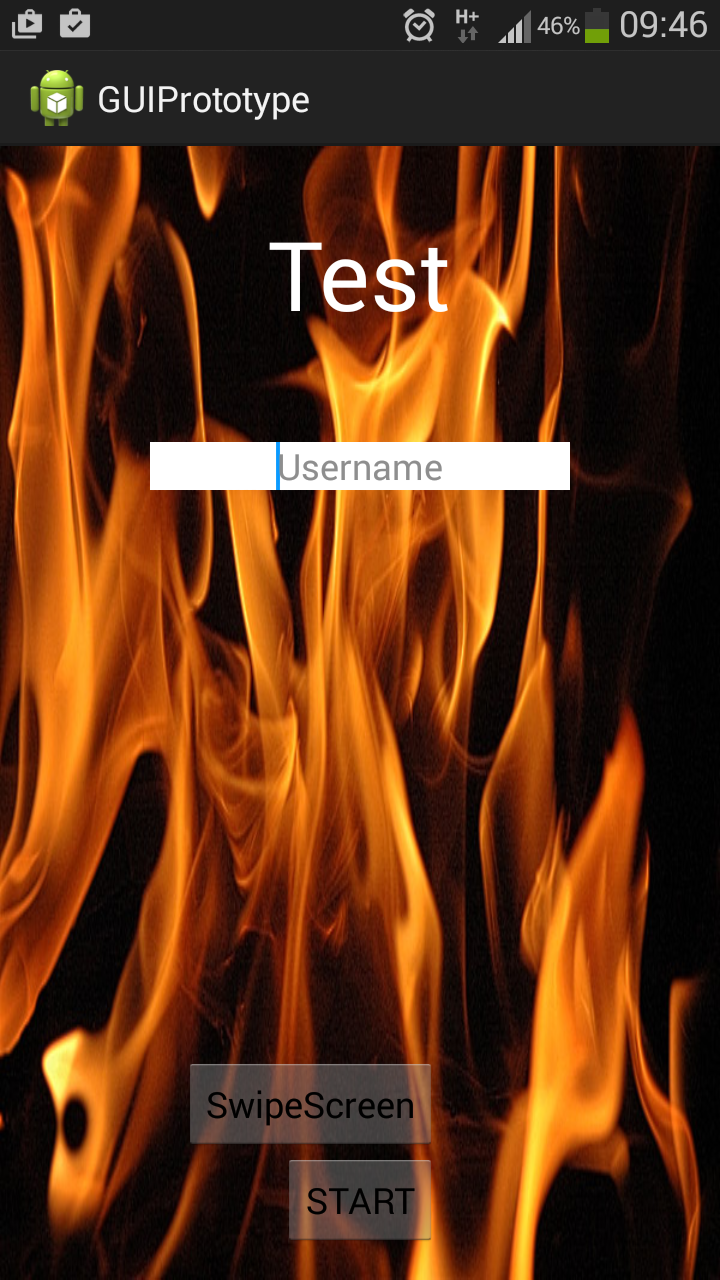
\includegraphics[width=0.48\textwidth]{4-Technische_Loesungen/4-5-GUI/Data/login_screen.png}
     \caption{Login Screen}
  \end{center}
\end{wrapfigure}


\subsection*{Swipe-Screen}
Schon in der sehr fr�hen Entwicklungsphase war festzustellen, das die verschiedenen Elemente der GUI - wie im folgenden weiter erl�utert- zu zahlreich sind, um sie auf einen Bildschirm umzusetzen. Die eigentliche Kartendarstellung w�re sonst zu klein gewesen. Also wurde entschieden die verschiedenen Elemente auf weitere Bildschirme zu verteilen. In den ersten entw�rfen geschah dies �ber einzelne Activities, also mehrere Bildschirme. Um gewisse Android Komfort-Funktionen und Gesten dem Nutzer zu verf�gung zu stellen wurden die zun�chst eigenst�ndigen Activites zu Fragments umgebeut, die dann in einem so genannten Swipe-Screen zusammengefasst werden. In diesem werden die Fragments als Tabs organisiert und der User kann entweder durch "`wischen"' (swipe) oder durch klicken auf die Tabs durch die GUI Navigieren. \newline
Ein weiterer Vorteil ist ebenfalls, dass benachbarte Tabs jeweils ein wenig {\color{red}'ein wenig' streichen} vorgeladen (Laden der Widgets) bzw. noch im Speicher behalten werden. Zum einen wird so sichergestellt, dass der Tab-Wechsel per wischen "`geschmeidig"' abl�uft, aber auch gibt es so nur sehr geringe Ladezeiten zwischen den einzelenen Bildschirmen. Zudem ist die von Google angepriesene "`Wiederverwendbarkeit"' von Fragments als UI (User Interface) ebenfalls n�tzlich, wenn weitere �hnliche Spiele umgesetzt werden sollen.

\begin{wrapfigure}{r}{0.5\textwidth}
  \begin{center}
    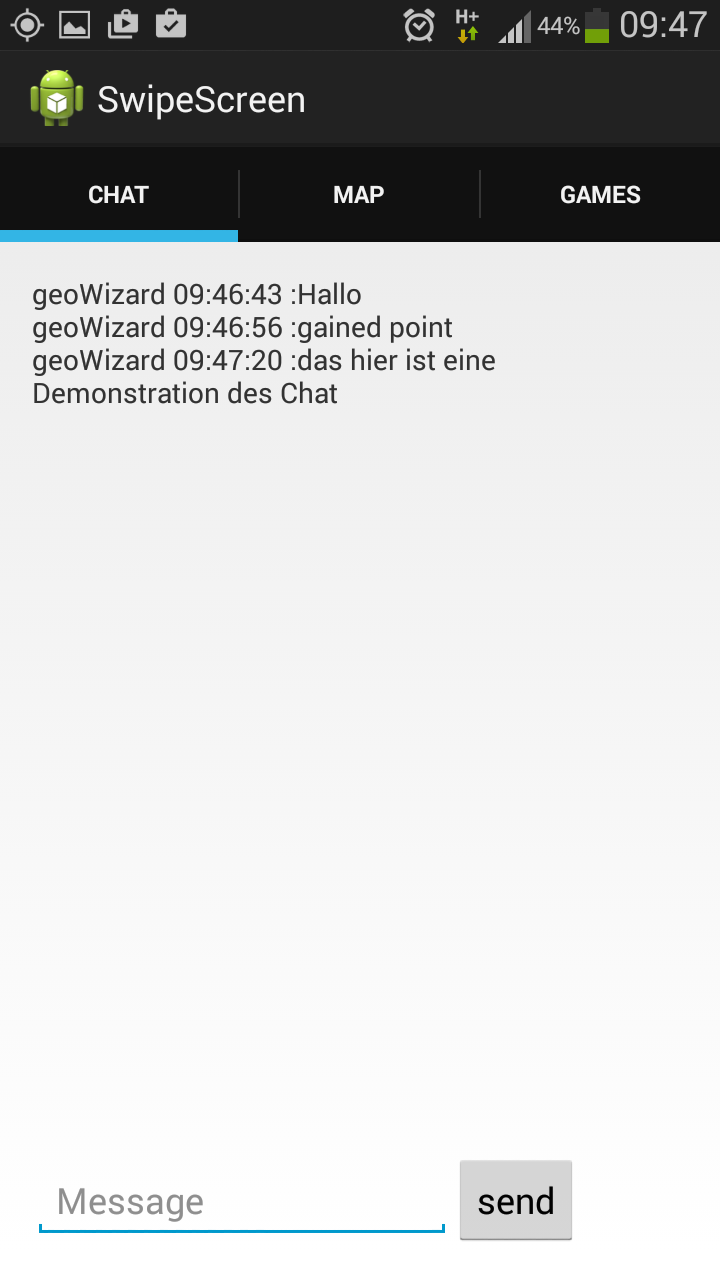
\includegraphics[width=0.48\textwidth]{4-Technische_Loesungen/4-5-GUI/Data/chat_screen.png}
     \caption{Chat Screen}
  \end{center}
\end{wrapfigure}

\subsubsection*{Chat-Screen}
In desem Fragment wird die m�glichkeit des Chattens zwischen mehreren Spielern umgesetzt. Die grafische Umsetzung des Chats wurde der von IRC (Instant Relay Chat) Clients nachempfunden und ist entsprechend simpel gel�st. Es wird der jeweilige Benutzername, Uhrzeit und die eigentliche Nachricht angezeigt. Die Eingabe der Chat-Nachricht erfolgt in einem Text-Eingabe-Feld. Die Anzeige der Chat-Nachrichten erfolgt in einem einfachen Textanzeige-Feld (TextView\footnote{{\color{red}\url{Link zur Android-Doku}}}) was wiederum in einem scrollbaren Feld (SrcollView\footnote{{\color{red}\url{Link zur Android-Doku}}}) liegt. Hierdurch ist es m�glich durch alle empfangenen Nachrichten "`durchzuscrollen"'. Wird eine Chat-Message (genaueres in Kapitel 4.4) empfangen, wird diese mittels Stringmanipulation an das Textfeld angeh�ngt. Hierbei ist zu beachten, dass die selbst verschickten Nachrichten erst an den Server gesendet werden und dann jeweils an die entsprechenden Nutzer. Somit kann es aufgrunde von �bertragungsverz�gerungen dazu kommen, das die eigene Nachricht verz�gert angezeigt, jedoch ist die korrekte Reihenfolge der Nachrichten gewahrt.

\newpage

\begin{wrapfigure}{r}{0.5\textwidth}
  \begin{center}
    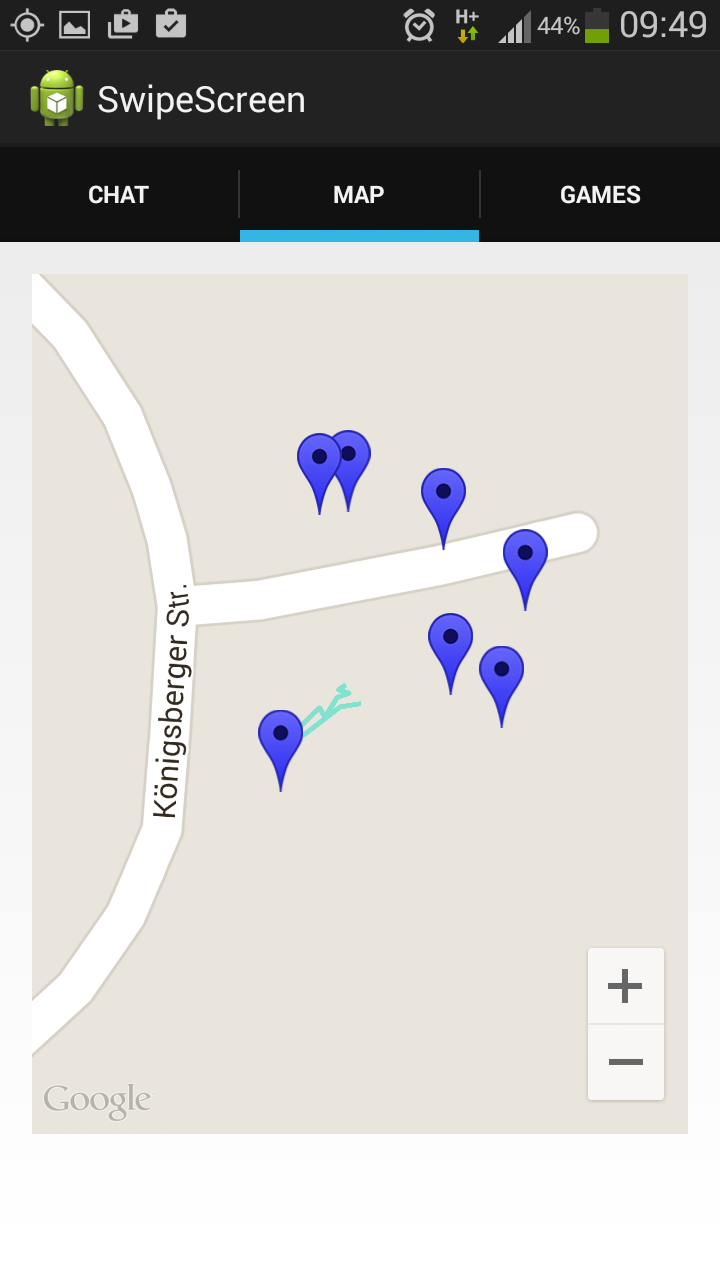
\includegraphics[width=0.48\textwidth]{4-Technische_Loesungen/4-5-GUI/Data/map_screen.png}
     \caption{Map Screen}
  \end{center}
\end{wrapfigure}

\subsubsection*{Map-Screen}
In diesem Fragment wird die Karte in einem weiterem Fragment angezeigt. Je nachdem welches Spiel gespielt wird zu zus�tzliche Widgets vorhanden, wie z.B. Interaktions Buttons, (Team-)Punkte anzeige usw.


\subsubsection*{Game-Screen}
In diesem Fragment werden momentan aktive Spiele angezeigt. Auch ist es m�glich neue Spiele zu erstellen. Die Anzeige der Liste der Spiele erfolgt in einer scrollf�higen Liste (ListView). Diese wird durch entsprechend angefordete Informationen �ber andere Spiele geupdatet. Diese Informationen werden durch Anfrage bei anderen Benutzer die sich eingeloggt haben �ber einen bestimmen Message-Typ abgerufen. Die Listen-Elemente sind interaktiv. Ein klick auf das entsprechende Spiel startet den beitritt. Um ein Spiel eines gewissen Typs zu Starten w�hlt man in einen Dropdown-Men� (bei Android Spinner) den entsprechenden Modus aus in klickt auf create. Man selbst betritt dieses Spiel und eintrag in der Spiele-Liste wird vorgenommen. 


\begin{figure}[r]  
    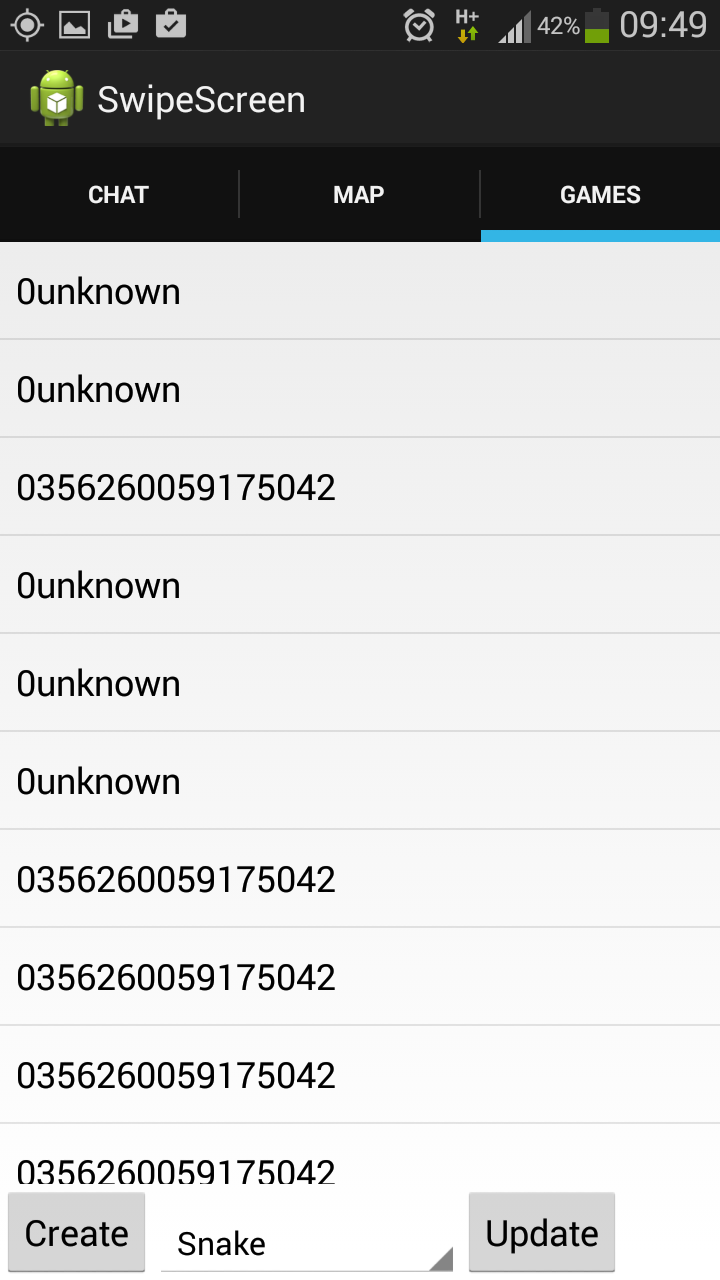
\includegraphics[width=0.48\textwidth]{4-Technische_Loesungen/4-5-GUI/Data/game_screen.png}
    \caption{Game Screen}
\end{figure}

\clearpage

\section{Sensorik}\label{sensorik}

\subsection*{BLEep}
BLEep bezeichnet eine Technologie, die Bluetooth Sender nutzt um Signale mit anderen Ger�ten auszutauschen. BLE (auch bekannt als Bluetooth Low Energy) sendet auf einer Frequenz von 2,4 GHz und nutzt Bluetooth Version 4.0, welche auch heute von allen g�ngigen Smartphones unterst�tzt wird.
Ein BLEep Sender wird an einem Ort angebracht und sendet dauerhaft Signale an alle umliegenden Ger�te. Die Reichweite des Senders liegt zwischen 15cm und 50m.
Mobile Ger�te empfangen das Signal und k�nnen an der Signalst�rke die Entfernung zum Sensor bestimmen. Je schw�cher das Signal, desto weiter ist die Entfernung.
Jeder BLEep Sensor besitzt eine ID, womit dieser sich eindeutig identifizieren l�sst.
Eine mobile Applikation empf�ngt also das Signal mit der ID und berechnet anhand der Signalst�rke die Entfernung. Aus diesem Kontext heraus k�nnen dann Interaktionen zwischen der mobilen App und dem Sensor durchgef�hrt werden. Dies ist auch mit mehreren Smartphones m�glich, denn die Sensoren haben keine Begrenzung hinsichtlich der Anzahl der Ger�te mit denen sie kommunizieren k�nnen. Auch kann ein Ger�t mit mehreren Sensoren gleichzeitig interagieren, was Spielraum f�r weitere m�gliche Szenarios l�sst.

\subsection*{Kompass}
Heute besitzen alle g�ngigen Smartphones eine Kompass-Funktionalit�t, die von mobilen Applikationen genutzt werden kann. 
Ganz allgemein richtet sich ein Kompass nach dem Magnetfeld der Erde. Er ist mit einer magnetischen Nadel ausgestattet, die sich auf den Nordpol einstellt.
In Smartphones ist ein kleines Magnetometer integriert, mit dem sich das Magnetfeld der Erde messen l�sst. Zudem bestimmt das Smartphone seine Position und Neigung anhand von anderer Sensorik. Das Ger�t kombiniert all diese Informationen und bestimmt somit die Richtung.

\subsection*{Geschwindigkeitsmessung}\label{geschwindigkeitsmessung}
Die Bewegungsgeschwindigkeit kann durch einen Be\-schleu\-ni\-gungs\-sen\-sor (auch Ac\-ce\-le\-ro\-me\-ter genannt) gemessen werden. Durch die auf ein Ger�t wirkende Tr�g\-heits\-kraft kann bestimmt werden ob eine Geschwindigkeitszunahme oder -abnahme stattfindet. Anhand der mittleren Erdbeschleunigung l�sst sich diese dann genau berechnen.
In modernen Smartphones ist solch ein Sensor verbaut. Dieser l�sst sich in mobilen Applikationen dazu benutzen um die Geschwindigkeit des Nutzers zu ermitteln.

Des weiteren kann auch durch GPS die Geschwindigkeit ermittelt werden. Moderne GPS-Ger�te speichern permanent ihre letzten Positionen. Somit k�nnen sie anhand der zur�ckgelegten Strecke mit Hinzunahme der ben�tigten Zeit ein recht genaues Geschwindigkeitsergebnis bestimmen.

\subsection*{Orientierung}\label{orientierung}
Smartphones sind in der Lage �ber die internen Sensoren etwas �ber ihre Ausrichtung zu erfahren. Hierbei werden das Accelerometer und das Magnetometer verwendet um eine Rotationsmatrix zu generieren.
Daraus kann dann die Orientierung Errechnet werden.

\subsection*{Thermometer}
Smartphones besitzen einen W�rmesensor, der genutzt werden kann um die Temperatur zu messen. Allerdings wird dieser meist durch die Betriebstemperatur beeinflusst und liefert daher nicht immer korrekte Werte f�r die Au�entemperatur. Aus diesem Grund werden die Messwerte von Thermometer Apps meist aus dem �rtlichen Wetterinformationsnetz bezogen. 
Die Innentemperatur hingegen wird tats�chlich durch den integrierten W�rmesensor bestimmt. Dazu muss das Ger�t sich aber eine gewisse Zeit im Standby Betrieb befinden, damit die Temperatur des Akkus das Ergebnis nicht verf�lscht.





\chapter{Projektarchitektur}

\section{Der Android Client}

\subsection{Aufbau der GUI}

GUIIIIIIIIIIIIIIIIIIIIIIIIIIIIIIIIIIIIIIIIIIIIIIIIIIIIIIIIIIIIIIIIIIIIIIIIIIIIIIIIIIIIIIIIIIIIIIII
IIIIIIIIIIIIIIIIIIIIIIIIIIIIIIIIIIIIIIIIIIIIIIIIIIIIIIIIIIIIIIIIIIIIIIIIIIIIIIIIIIIIIIIIIIIIIIIIII
IIIIIIIIIIIIIIIIIIIIIIIIIIIIIIIIIIIIIIIIIIIIIIIIIIIIIIIIIIIIIIIIIIIIIIIIIIIIIIIIIIIIIIIIIIIIIIIIII

\subsection{Kommunikation}

blablablablablablablablablab lablablablabla blablablabla blablablablablablab  lablablablab lablablablab labla
blablablablablab lablablablablablablabla blablablablablablablablablablablablab lablablablablabl ablablabla
blablablablablablablablablablablablablablablablablablablablablablablablablablablablablablablablablabla
blablablab lablablablabla blablablablablablablabl  ablablablablablablablablabl ablabla blablablablablablabla
blablablablablablablablablablablablablablablablablablablablablablablablab lablablablablablablablablabla
blablablablablablabla blablablablablablablablablablablablablablablablablablablablablablablablablablabla
blablablablablablablablablablablablablablablablablablablab lablablablablablablablablabla  blablablablabla
blablablablablablablablablablablablablablablablablablablablablablablablablablablablablablablablablabla
blablablablab lablablablablablabl ablablablablablablablablablablablablablablablablablablablablablablabla
blablablablablablablablablablablablablablablablablablab ablablablablablablabl ablablablablablablablabla
\subsection{Die Karte}

\input{5-_Projektarchitektur/5-1_Der_Android_Client/5-1-3_Die_Karte/5-1-3-1_OpenStreetMap_vs_GoogleMaps/OSM_vs_GMS.tex}
\input{5-_Projektarchitektur/5-1_Der_Android_Client/5-1-3_Die_Karte/5-1-3-2_Fazit/OSM_vs_GMS_Fazit.tex}
\subsection{Die Karte}

\input{5-_Projektarchitektur/5-1_Der_Android_Client/5-1-4_GPS/5-1-4-1_LocationManager_vs_LocationClient/LM_vs_LC.tex}
\input{5-_Projektarchitektur/5-1_Der_Android_Client/5-1-4_GPS/5-1-4-2_Fazit/LM_vs_LC_Fazit.tex}
\subsection{Spiellogik}

Lebe lange und in Frieden.

\section{Snake}


\subsection*{Spielidee}
Das zweite Spiel, das von uns umgesetzt wurde, ist ein Flaggenspiel. Hierbei handelt es sich um eine Abwandlung von Capture the Flag. Es wird mit Stealth-Elementen erweitert und die Spielmechanik des Ausschaltens von Gegnern ist anders gel�st. Dieses Spiel sollte nach M�glichkeit in einer Stadt gespielt werden, da es wichtig ist in einer Menge von Passanten m�glichst unerkannt zu bleiben. Es gibt zwei Teams, die jeweils eine Basis haben. Basen werden jeweils von dem Mitglied eines Teams erstellt, welches als erstes die Erstellung �ber einen Button ausl�st. Hierbei wird als Zentrum der Basis die aktuelle Position des entsprechenden Spielers genommen. Beim betreten des Spiels, k�nnen sich Spieler zwischen Team Blau und Team Rot entscheiden. Die eigene Flagge erscheint in der N�he der eigenen Basis. Die Position der eigenen Flagge ist den Teammitgliedern unbekannt, man sieht nur die Position der gegnerischen Flagge. Die Flaggen sollen nur auf Stra�en bzw. Gehwegen (nicht in Geb�uden) zuf�llig platziert werden. Diese Platzierung wird vom Server �ber Bilderkennung bestimmt. So wird die Erreichbarkeit der Flaggen sichergestellt. Als Spieler sieht man nur die Positionen der eigenen Teammitglieder. Zur Organisation kann der Chat verwendet werden. Es ist m�glich die n�here Umgebung nach Gegnern zu scannen. Die gescannten Gegner sind dann f�r kurze zeit sichtbar. Dieses Scan-Verfahren ist jedoch nicht dauerhaft verf�gbar, sondern erst wieder m�glich nach l�ngerer Abklingzeit. Es ist m�glich potentielle Gegner zu markieren. Die Reichweite beim Markieren ist begrenzt und Richtungsabh�ngig. Hierbei wird das Smartphone auf den potentiellen Feind ausgerichtet und ein Mark-Button gedr�ckt (Auch hier besteht eine gewisse Abklingzeit). Ist dieser ein gegnerischer Mitspieler wird er markiert und ist f�r l�ngere Zeit auf der Karte sichtbar. Der Betroffene bekommt �ber seine Markierung keine R�ckmeldung. Ein Spieler, der sich in der N�he der gegnerischen Flagge befindet, kann diese aufnehmen. Um einen Spiel-Punkt zu erreichen muss die aufgenommene Flagge zur eigenen Basis gebracht werden. Dem Gegnerteam wird die Position angezeigt, an der die Flagge aufgenommen wurde. Wird ein Flaggentr�ger markiert, verliert er die Flagge und sie erscheint an einer neuen zuf�lligen Position. War der Flaggentr�ger vor der Aufnahme markiert, so ist er mit Flagge zu sehen. Wenn ein Spieler eine bestimmte Geschwindigkeit �berschreitet, wird er ebenfalls f�r das Gegnerteam sichtbar. Somit haben schnellere L�ufer keinen direkten Vorteil.
\begin{figure}
	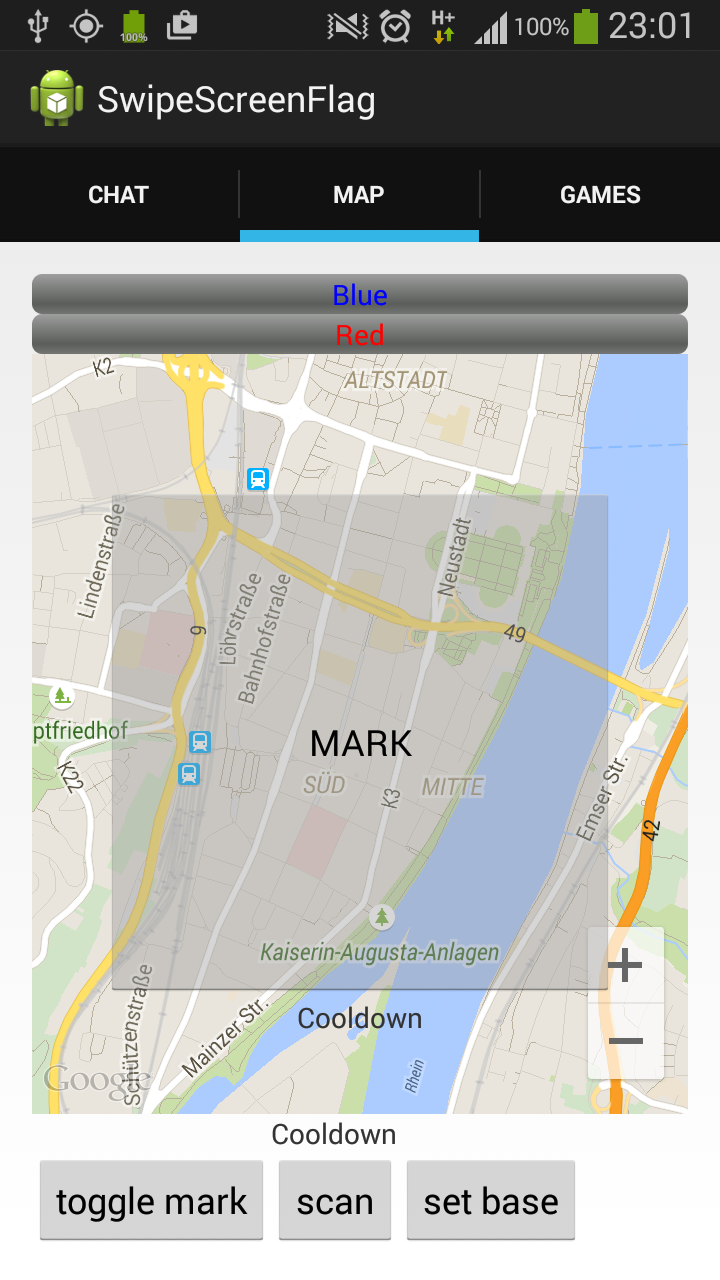
\includegraphics[width=0.5\textwidth]{5-Implementation_von_Beispielapps/5-2-Verstecken/Data/map_screen_mark_on.png}
	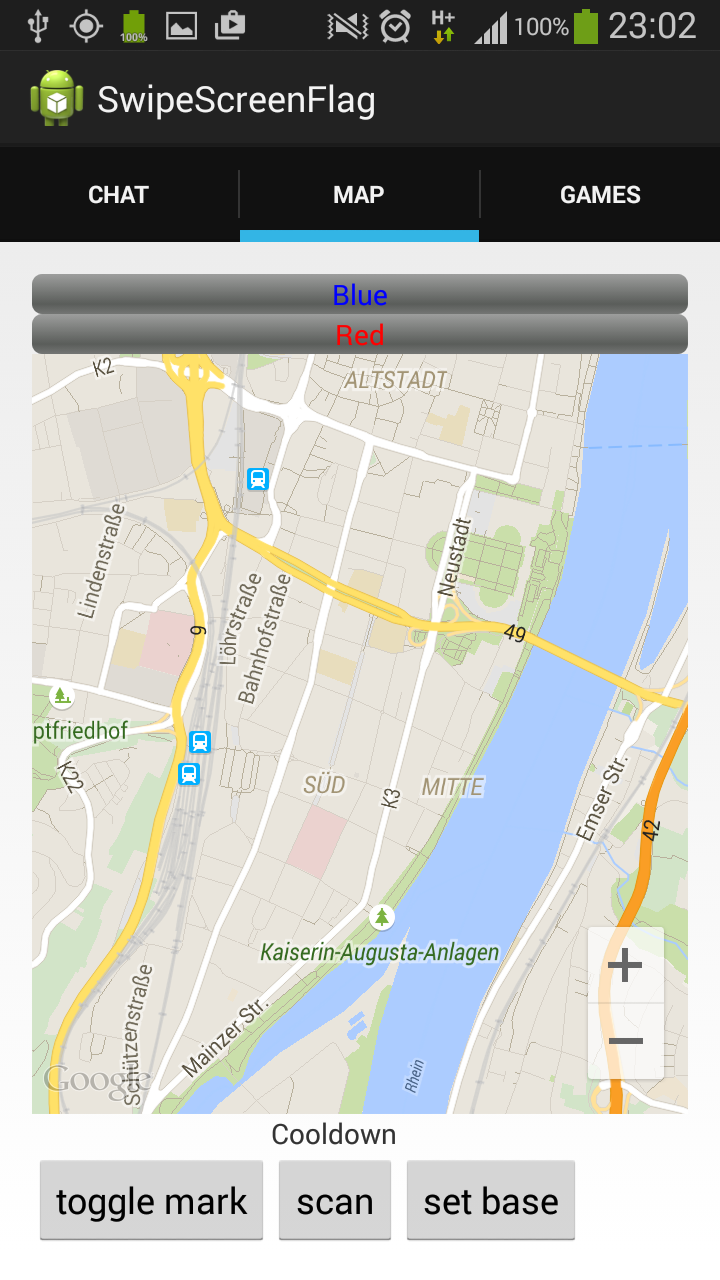
\includegraphics[width=0.5\textwidth]{5-Implementation_von_Beispielapps/5-2-Verstecken/Data/map_screen_mark_off.png}
	\caption{Map-Screen mit Mark-Button (rechts) Map-Screen ohne Mark-Button (Links)}
	\label{fig:flaggmap}
\end{figure}


\subsection{Spiellogik}

\subsubsection*{Server}
Der Server wird hier noch mit einer Zusatzfunktion ausgestattet. Er generiert nach vorher festgelegten Bedingung g�ltige Flaggenpunkte. In diesem Fall z�hlen Stra�en als g�ltige Punkte. Der Server ruft �ber GoogleStaticMap einen Kartenabschnitt ab, auf dem der Flaggenpunkt generiert werden soll. Nun wird ein zuf�lliger Pixel in der Mitte des Bildes nach der Farbe �berpr�ft. Stimmt dieser mit der Farbe von Stra�en �berein, wird diese Position als g�ltig zur�ck �bertragen und der Flaggenpunkt kann generiert werden. Ist die Farbe ung�ltig wird ein entsprechender neuer Kartenabschnitt aufgerufen und die Prozedur beginnt erneut.

\subsubsection*{Client}
Auf der Client-Seite wird die Sichtbarkeit der Spieler und Objekte (Flaggen und Basen) gehandhabt.

\paragraph{Markieren}
 S�mtliche Positionen sind den Gerten bekannt, aber nicht alle sichtbar. Damit verbunden sind auch die Funktionalit�ten des Markieren und Scannens. F�r das Markieren werden jeweils die beiden Koordinaten des Markierenden (A) und des Markierten (B), sowie den Sichtkegel von A und eine Reichweite ben�tigt. 
F?r den Sichtkegel ben�tigt man einen Orientierungswinkel ($\alpha$), welche mittels der Sensoren f�r Orientierung (s. \ref{orientierung}) ermittelt wird, sowie einen vorher festgelegten Winkel f�r den Sichtbereich ($\beta$). Nun wird der Winkel der beiden Punkte A und B ($\gamma$) bestimmt (s. \ref{abstandsmessung}).


Liegt $\gamma$ im Intervall $[ \alpha - \frac{\beta}{2}; \alpha + \frac{\beta}{2}]$ und ist die Distanz zwischen A und B innerhalb der Reichweite, so gilt B als markiert. �ber eine Nachricht wird den anderen Teammitgliedern mitgeteilt das B jetzt markiert und somit f�r eine gewisse Zeit sichtbar ist. A kann f�r eine vordefinierte Zeit keine weiteren Gegner markieren.

\paragraph{Scannen}

Um einen festgelegten Radius eines Spielers nach Gegnern zu scannen, wird die Distanz (s. \ref{abstandsmessung}) zwischen dem Scannenden (C) und allen gegnerischen Spielern ermittelt. C werden, f�r eine kurze Zeit, alle gegnerischen Spieler angezeigt, die sich innerhalb eines bestimmten Distanzwertes befinden. Die M�glichkeit zu Scannen steht C f�r eine gewisse Zeit nicht mehr zur Verf�gung.

\paragraph{Geschwindigkeits�berpr�fung}
Es existiert eine st�ndig aktive Geschwindigkeits�berpr�fung der Spieler durch ihre Koordinaten (s. \ref{locationManager}). Wenn eine feste Maximalgeschwindigkeit durch einen Spieler �berschritten wird, schickt der entsprechende Client eine Nachricht an alle gegnerischen Ger�te, dass dieser angezeigt werden soll. Wird die Maximalgeschwindigkeit wieder unterschritten, ist der Betroffene wieder unsichtbar f�r die Gegner

\paragraph{Basen- und Flaggenplatzierung}
Die Basis eines Teams wird vom ersten Teammitglied gesetzt, welches auf den "`set Base"' Button klickt. Als Zentrum wird die momentane Position des Spielers genommen. Die Darstellung erfolgt als Kreis. Nun wird in einem vorher festgelegtem Radius um die Basis zuf�llig die Teamflagge platziert. Die Auswahl f�r eine g�ltige Koordinate trifft dabei der Server und teilt dies den entsprechenden Mitspielern �ber eine Nachricht mit. Die aktuelle Position der Flagge wird jedoch dem eigenen Team nicht angezeigt. Wird die Flagge von einem Mitspieler des gegnerischen Team gestohlen, werden die betroffenen Spieler �ber einen Vibrationsalarm informiert. Auch wird die letzte Position der Flagge vorl�ufig angezeigt. Wenn der Flaggentr�ger gestoppt wird, generiert der Server wieder eine g�ltige Position f�r eine neue Flagge 
\subsection*{Umgesetzte Features}
%aaaaaaaaarg gkls akj dasdlj ad ka kd askd 
Zus�tzlich zu den im Zuge der Implementation von Snake umgesetzten Features wurde die Geschwindigkeitsmessung (siehe Abschnitt \ref{sec:geschwindigkeitsmessung}) implementiert. F�r das Markieren wurde au�erdem eine Richtungsangabe (siehe Abschnitt \ref{sec:richtungsangabe}) ben�tigt.
\section{Noch bestehende Bug}

Waaaaaaaaaaaaaaaaaaaaaaaaaaaaaaaaaaaaaaaaaaaaaaaah Insekten holt das Insektenspray

\chapter{Fazit}
Es ist uns gelungen, ein klassisches Computerspiel so umzusetzen, dass die physische Umgebung der Teilnehmer als Spielfeld bzw. Map dient. Die Qualit�t des GPS-Sensors der verwendeten Handys kann hierbei jedoch die Steuerung hakelig erscheinen lassen und so den Spielspa� beeintr�chtigen. 
%So muss das Spielfeld gen�gend gro� sein und  Spieler m�ssen Acht geben keine zu scharfen Kurven zu laufen und d�rfen sich nicht zu schnell bewegen. 
Da in derzeit gebr�uchlichen Ger�ten gravierend unterschiedlich pr�zise Sensoren verbaut sind, kann man auf eine gro�e Verbreitung zuverl�ssiger Sensoren in der Zukunft hoffen. Durch pr�zisere Positionsbestimmung k�nnten Spiele mit schneller Bewegung auf kleinerem Raum fl�ssig spielbar werden.
\chapter{Ausblick}

%\section{Weitere Features}
F�r die Zukunft ist zu erwarten, dass es mit Hilfe neuartiger Ger�te m�glich sein wird, virtuelle Realit�t und tats�chliche Umgebung noch mehr verschmelzen zu lassen, als es heute machbar ist. 
Einen vielversprechenden Ansatz bietet Google Glass, ein Minicomputer, der an eine Brille montiert Informationen in das Sichtfeld des Benutzers einblendet. Google Glass ist ein Paradebeispiel f�r \textit{augmented reality}.
Die zweite und dritte Generation dieses Ger�tes sind derzeit in der Entwicklung \cite{cb}.
Google Glass eignet sich f�r die Umsetzung von Snake oder anderen Spielen in die reine Realit�t. Dadurch, dass das Ger�t am Kopf getragen wird und die Informationen direkt in das Sichtfeld eingeblendet werden, ist es nicht mehr n�tig w�hrend dem Spiel st�ndig auf das Smartphone zu schauen. 
% ?? Da das Spiel im Freien gespielt wird, erh�ht sich die Sicherheit des Nutzers wesentlich.
Des Weiteren k�nnen die Positionen von Wegpunkten und anderen virtuellen Objekten pr�ziser und dreidimensional in der Realit�t dargestellt werden, als es auf einem kleinen Smartphone Display der Fall ist. 
% ?? Zus�tzlich hat der Spieler die H�nde frei, was mehr M�glichkeiten bietet, wie er mit den virtuellen Objekten interagieren kann.

Microsoft HoloLens \footnote{\url{https://www.microsoft.com/microsoft-hololens/en-us/experience}} ist ein weiteres Ger�t, das virtuelle und reine Realit�t vermischt. Der Ansatz ist aber derzeit nur auf geschlossene R�ume beschr�nkt.
Hologramme werden in das Sichtfeld des Benutzer eingeblendet, so dass man mit virtuellen und reellen Objekten gleichzeitig interagieren kann. 
%Microsoft wirbt damit, sowohl den Alltag zu Hause, als auch das produktive Arbeiten zu vereinfachen.
%F�r das Snake-Spiel im Freien ist HoloLens derzeit nicht geeignet. 
Sobald diese Augmented-Reality-L�sungen ausgereift sind, ergeben sich eine ganze F�lle an M�glichkeiten f�r interaktive Spiele.

Oculus Rift\footnote{\url{https://www.oculus.com/}} ist ein Ger�t f�r die vollst�ndig visuelle virtuelle Realit�t. An die Augen gelangen keine realen Eindr�cke mehr. Rift ist ungeeignet f�r ein Spiel im Freien. Google stellt aber im Rahmen seiner Maps und Street View Dienste dreidimensionale Ansichten von St�dten und Sehensw�rdigkeiten bereit\footnote{\url{https://support.google.com/maps/answer/3092441?hl=de}}.
Hier k�nnte es in Zukunft m�glich sein, solche Daten in Anwendungen f�r Rift zu verarbeiten. So w�re es m�glich, sich im Snake-Spiel virtuell durch der Realit�t nachempfundene R�ume zu bewegen.
\section{Weitere Spiele}
M�gen die Spiele beginnen





\clearpage
\newpage
\nocite{*}
\bibliographystyle{alphadin}
\bibliography{literatur}


\end{document}